% Patch für LaTeX laden:
%\RequirePackage{fixltx2e}

%------------------------------------------------------------------------------
%---------------- Docmentenklasse, Layout und Ränder: -------------------------
%------------------------------------------------------------------------------

\documentclass[
        paper=a4,               % Papierformat DIN A4
        fontsize=12pt,
        BCOR=12mm,              % 12mm Binderandkorrektur
        parskip=half,           % Absätze als halbe Leerzeile
        headsepline,            % Linie zwischen Kopfzeile und Dokument
        cleardoublepage=plain,  % Keine Kopf/Fußzeile auf Leerseiten
        bibliography=totoc,     % Bibliographie als nicht-nummeriertes 
                                % Kapitel im Inhaltsverzeichnis
        open=right,             % Kapitel beginnen immer aufrechten Seiten
        %open=any,               % Kapitel dürfen auf beiden Seiten beginnen
        numbers=noenddot,       % Keine Punkte nach Abbildungsnummern
        captions=tableheading,  % Spacing für Captions über Tabellen an
        titlepage=firstiscover, % Titelseite ist Deckblatt, symmetrische Ränder
        headings=normal,         % kleinere Überschriften
        %draft,
    ]{scrbook}


% Warnung, falls erneut kompilirt werden muss:
\usepackage[aux]{rerunfilecheck}

% Beschränkung auf chapter und section im Inhaltsverzeichnis:            
\setcounter{tocdepth}{2}

%------------------------------------------------------------------------------
%------------------------------ Sprache und Schrift: --------------------------
%------------------------------------------------------------------------------

% Deutsche Spracheinstellungen
%\usepackage{polyglossia}
%\setdefaultlanguage{german}
\usepackage[ngerman]{babel}

% stellt den \enquote{} Befehl

% verbessert das allgemeine Schriftbild:
\usepackage{microtype}

\usepackage{fontspec}
\defaultfontfeatures{Ligatures=TeX}


\usepackage{xcolor}

% Astroparticle shortcuts
\usepackage{hepnicenames}
\usepackage{isotope}


%------------------------------------------------------------------------------
%------------------------ Für die Matheumgebung--------------------------------
%------------------------------------------------------------------------------

\usepackage{amsmath}
\usepackage{amssymb}
\usepackage{mathtools}

% Enable Unicode-Math and follow the ISO-Standards for typesetting math
\usepackage[
  math-style=ISO,
  bold-style=ISO,
  sans-style=italic,
  nabla=upright,
  partial=upright,
]{unicode-math}
\setmathfont{Latin Modern Math}
\usepackage[autostyle=true,german=quotes]{csquotes}

% schöne Brüche im Text mit \sfrac{}{}
\usepackage{xfrac}  


%Gleichungsnummern Kapitel.Unterkapitel.Gleichung
\renewcommand{\theequation}{\thesection{}.\arabic{equation}}
\numberwithin{equation}{chapter}
\numberwithin{equation}{section}

\newcommand{\ab}{\\\\}
\newcommand{\qa}[1]{\textbf{#1}\mbox{}\\}
\newcommand{\absatz}{\\\\}
\newenvironment{qanda}{\setlength{\parindent}{0pt}}{\bigskip}
\newcommand{\Q}{\bigskip\bfseries}
\newcommand{\A}{\par\textbf{} \normalfont}

%------------------------------------------------------------------------------
%---------------------------- Einheiten ---------------------------------------
%------------------------------------------------------------------------------

\usepackage[
  locale=DE,
  separate-uncertainty=true,
  per-mode=symbol-or-fraction,
]{siunitx}
\sisetup{math-micro=\text{µ},text-micro=µ}

%------------------------------------------------------------------------------
%------------------------------ Tabellen: -------------------------------------
%------------------------------------------------------------------------------

\usepackage{booktabs}       % stellt \toprule, \midrule, \bottomrule
\usepackage{threeparttable} % für komplexere Tabellen

%------------------------------------------------------------------------------
%------------------------------ Grafiken: -------------------------------------
%------------------------------------------------------------------------------

\usepackage[]{graphicx} % enhances includegraphics
\usepackage{grffile}  % adds support for a larger range of file names

\usepackage{scrhack}
\usepackage{float}
\floatplacement{figure}{htbp}
\floatplacement{table}{htbp}

\usepackage{caption}
\captionsetup{%
            labelfont=bf,               % Label fett
            format=plain,               % Caption-Text steht auch unter "Tabelle x"
            width=0.9\textwidth,        % Bereich für Caption schmaler als für Text
            font=small,
           }

\usepackage{subcaption}   % for subfigures
%\usepackage{rotating}
%\usepackage[above,below,section]{placeins} % forces floating objects to stay within a given border
%\usepackage{flafter}  % floats only appear after they are referenced


%------------------------------------------------------------------------------
%------------------------------ Bibliographie ---------------------------------
%------------------------------------------------------------------------------

\usepackage[%
    backend=biber,
    style=alphabetic,]{biblatex}    % Biblatex mit biber
    \addbibresource{content/references.bib}     % die Bibliographie einbinden
\DeclareBibliographyAlias{misc}{article}
\DefineBibliographyStrings{german}{andothers = {{et\,al\adddot}}}


%------------------------------------------------------------------------------
%------------------------------ Sonstiges: ------------------------------------
%------------------------------------------------------------------------------



\usepackage[pdfusetitle,unicode]{hyperref}
\usepackage{bookmark}
\usepackage[shortcuts]{extdash}
\usepackage{bbding} % used for \XSolidBrush x
\usepackage{pdflscape}
% forbid typographic malpractice
\clubpenalty = 10000
\widowpenalty = 10000
\displaywidowpenalty = 10000

\renewcaptionname{ngerman}\sectionautorefname{Abschnitt}
\renewcaptionname{ngerman}\chapterautorefname{Kapitel}
\renewcaptionname{ngerman}\subsectionautorefname{Unterabschnitt}
\renewcaptionname{ngerman}\figureautorefname{Abbildung}

%------------------------------------------------------------------------------
%-------------------------    Angaben zur Arbeit   ----------------------------
%------------------------------------------------------------------------------

%Titel der Arbeit
%\newcommand{\thetitle}{Multivariate Selektion atmosphärischer Myon-Neutrinos im Energiebereich $4 - \SI{190}{\giga\electronvolt}$ mit IceCube DeepCore}
\newcommand{\thetitle}{Betrachtung technischer Maßnahmen zur Umsetzung ethischer Sicherheitsaspekte bei der Erstellung und Anwendung von Reinforcement-Learning-Modellen}
\newcommand{\Jahr}{2020}
\newcommand{\Geburtsort}{Paderborn}
\newcommand{\Lehrstuhl}{Experimentelle Physik V}
\newcommand{\Betreuer}{Prof. Dr. Sebastian Bab}
\newcommand{\Zweitgutachter}{Prof. Dr. Burkhard Lenze }
\newcommand{\Abgabedatum}{\today}


%Author und Email-Adresse
\author{
    Niels Schlunder\\
    geboren in \Geburtsort
}

\titlehead{
    
\includegraphics[height=2cm]{logos/FH_Dortmund-logo.pdf}
}
\title{\thetitle}
\date{\Jahr}

%\subject{Arbeit zur Erlangung des akademischen Grades\\ Master of Science}
\publishers{Praktische Informatik \\ Fachbereich Informatik \\ Fachhochschule Dortmund}



\begin{document}
\frontmatter
\maketitle
%Gutachterseite
\thispagestyle{empty}
\vspace*{\fill}
\begin{tabbing}
2. Gutachter : \=\kill
1. Gutachter : \> \Betreuer \\[11pt]
2. Gutachter : \> \Zweitgutachter \\[11pt]
\end{tabbing}
\vspace{11pt}
Abgabedatum: \Abgabedatum
\newpage

\renewcommand{\baselinestretch}{1.5}\normalsize
% hier beginnt der Vorspann, nummeriert in römischen Zahlen
\thispagestyle{plain}
\section*{Kurzfassung}
Reinforcement Learning wird als Kerntechnologie in autonomen Anwendungen der Medizin, Mobilität oder unbemannten Waffensystemen eingesetzt.
Daraus ergibt sich neben dem Potenzial gesellschaftlichen und wissenschaftlichen Fortschrittes auch das Risiko zur Gefährdung von Wohlergehen und Würde des Einzelnen.
Basierend auf Prinzipien der angewandten Ethik und der Betrachtung regionaler Leitlinien für ethische KI-Anwendungen werden im Rahmen dieser Arbeit ethische Werte als Grundlage für moralisches Handeln von Reinforcement Learning Agenten definiert.
Um die Umsetzung dieser Werte zu unterstützen wird ein Vorgehensplan aufgezeigt, der parallel zu gängigen Vorgehensmodellen in den Entwicklungsprozess eingeführt werden kann.
Innerhalb des Vorgehensplan werden technische und organisatorische Maßnahmen eingeführt, die über den tatsächlichen Implementierungsprozess hinaus die Zusicherung moralischen Handelns von Reinforcement Learning Agenten unter Miteinbeziehung aller Projektbeteiligten und möglichst verfahrensunabhängig unterstützt.  

\section*{Abstract}
Reinforcement Learning as a core technology for autonomous applications can be used in domains such as healthcare, transport or unmanned weapon systems.
Apart from the potential for social and economic growth, the technology could possbily endanger human dignity and well-being.
Based on principles of applied ethics and regional guidelines for ethical AI applications, ethical values as a foundation for moral behaviour of Reinforcement Learning agents are defined.
To support the implementation of these values, process guidelines are proposed, which can be introduced simultaneous to most existing process models.
The guidelines contain technical and organisational measures as a mostly methodological independent approach, which ensures moral behaviour of Reinforcement Learning agents beyond the implementional process including all project members.
\tableofcontents

\mainmatter
% Hier beginnt der Inhalt mit Seite 1 in arabischen Ziffern
% Introduction
% Theory: Astro physics, cosmic rays: interactions in the atmosphere, Flux models; IceCube: DeepCore, Measurement, Reconstruction, Weighting
% Analysis: data preparation: weighting, remove garbage; feature generation; feature selection; separation; validation; evaluation
% Conclusion and outlook
\chapter{Einleitung} \label{chap:einleitung}
Reinforcement Learning als maschinelles Lernverfahren ermöglicht eine vielversprechende Herangehensweise an die Entwicklung autonomer Systeme.
Es unterscheidet sich zu anderen maschinellen Lernverfahren, indem keine Kenntnis über die Klassenzugehörigkeit der Daten benötigt wird.
Insbesondere für die Anwendung in autonomen Systemen ist es z.B. bei überwachten Lernverfahren aufwendig, genügend große Datenmengen zu erzeugen, speziell dann, wenn alle Anwendungsfälle abgedeckt und eindeutig einer Klasse zugewiesen werden müssen.
Im Vergleich zu herkömmlichen Paradigmen bietet Reinforcement Learning die Möglichkeit zur selbständigen Anpassung und Generalisierung an fremde Situationen. 
Durch diese Potenzial besteht wirtschaftliches und politisches Interesse am Fortschritt, weshalb es umso wichtiger ist, eine sachliche Diskussion bezüglich der Nutzung und möglicher Bedenken zu führen.
Ein verantwortungsvoller Umgang bietet dann Potenzial für wirtschaftlichen und gesellschaftlichen Fortschritt.
Denn auch wenn die technischen Möglichkeiten vielversprechend aussehen, müssen bei allen lernenden Systemen neben ethischen Bedenken des Nutzungskontextes auch Bedenken während des Entwicklungsprozesses betrachtet werden, denn Fehlentscheidungen können fatale Folgen \cite{amodei2016}\cite{hawkins} haben und so das Wohl und die Würde des Menschen gefährden.
Es stellen sich deshalb die Fragen, welche Maßnahmen ergriffen werden können, damit Agenten zu unserem Wohl gemäß unserer Werte handeln, wie diese Werte formalisiert werden können und wie Adaption und Akzeptanz innerhalb der Gesellschaft zugesichert werden kann.
\ab 
Im Rahmen dieser Arbeit soll ein Vorgehensplan zur Umsetzung technischer und organisatorischer Maßnahmen erstellt werden, um ethisches Bedenken in bestehende Prozesse der Entwicklung von Reinforcement-Learning-Anwendungen zu integrieren.
Dafür werden zunächst Grundlagen des Reinforcement Learning als Kerntechnologie dieser Arbeit eingeführt.
Um nicht von einer einzelnen Technologie abhängig zu sein wird dafür der Markov-Entscheidungsprozess als Grundlage zur Umgebungsmodellierung, sowie allgemeine Begriffe und Eigenschaften eingeführt, wodurch eine eigene Evaluation der Technologie gemäß des Nutzungskontexts erfolgen kann.
Da im Rahmen der Arbeit Werte zum moralischen Handeln von Reinforcement-Learning-Agenten definiert und technische Maßnahmen zur Umsetzung dieser Werte aufgezeigt werden, wird anschließend ein Überblick über Grundlagen der angewandten Ethik und Moral, sowie der Maschinenethik als Bereichsethik gegeben und diskutiert, inwiefern Reinforcement-Learning-Agenten moralisch handeln können.
Anschließend werden als Grundlage der Definition der ethischen Werte die Maßnahmen zur Zusicherung ethischen Umgangs mit Künstlicher Intelligenz auf internationaler, europäischer und asiatischer Ebene, und der USA betrachtet. 
In \autoref{chap:diskussion} wird dann zunächst der Kontext der Arbeit abgegrenzt, Anwendungsgebiete sowie der Stand der Technik betrachtet und mit dieser Arbeit verglichen, sowie Herausforderungen bei der Konzeption technischer Maßnahmen ethischer Reinforcement-Learning-Anwendungen als Evaluationsgrundlage diskutiert.
In der eigentlichen Konzeption in \autoref{chap:konzeption} wird zunächst die Wahl ethischer Werte als Grundlage für die Erstellung des Vorgehensplan basierend auf den ethischen Grundlagen und der regionalen Maßnahmen begründet.
Anschließend wird in \autoref{sec:massnahmen} der eigentliche Vorgehensplan vorgestellt. 
Der Vorgehensplan ist angelehnt an einen generischen Softwareentwicklungszyklus \cite[S. 64]{broy2013}, zeigt technische und organisatorische Maßnahmen zur Umsetzung der ethischen Werte auf und beschreibt Möglichkeiten die in \autoref{sec:Herausforderungen} genannten Herausforderungen zu lösen.
Abschließend wird der Vorgehensplan gemäß der definierten Fragestellungen, den regionalen Maßnahmen der Länder und den Herausforderungen evaluiert, sowie abschließend zusammengefasst und ein Ausblick über mögliche zukünftige Weiterentwicklungen diskutiert.
\chapter{Grundlagen des Reinforcement Learning}\label{chap:grundlagen_rl}
Autonome Systeme bieten die Möglichkeit zur selbständigen Lösung komplexer oder für Menschen gefährlicher Probleme in potenziell unbekannten Umgebungen. 
Die technische Umsetzung dieser Systeme durch klassische Programmierparadigmen ist in vielerlei Hinsicht problematisch.
So ist der Zustandsraum in realen Anwendungen extrem groß. 
Insbesondere in fremden Umgebungen mangelt es klassischen Programmen an Allgemeingültigkeit. 
Das System sollte das Problem auch in unbekannten Umgebungen lösen können, ohne dass eine Anpassung der Logik notwendig ist.
Als zusätzliche Stufe der Komplexität ergibt sich zudem die Interaktion mit Menschen oder anderen autonomen Systemen. 
\ab
Menschen lernen von früh auf, indem sie den Einfluss ihrer Aktionen auf die Umgebung \cite[S. 1]{sutton2018} beobachten und daraus Schlüsse ziehen.
Jede Reaktion der Umwelt auf das Verhalten wird verarbeitet und beeinflusst die spätere Wahl der Aktionen.
Der Mensch entwickelt sich dadurch im Laufe der Zeit \cite[S. 634]{castano}.
Formal sind viele Reinforcement-Learning-Verfahren angelehnt an das psychologische Phänomen der operanten Konditionierung \cite[S. 34]{lefrancois1986}. 
Laut Skinner wird operante Konditionierung folgendermaßen beschrieben: 
\enquote{Wenn eine Reaktion [...] von einer Verstärkung gefolgt wird, so resultiert daraus eine Erhöhung der Wahrscheinlichkeit, dass diese Reaktion später unter ähnlichen Umständen wieder auftritt.}\cite[34]{lefrancois1986}.
Analog dazu sinkt die Wahrscheinlichkeit, wenn die Aktion bestraft wird.
Das Ausprobieren von Aktionen erfolgt nach dem Versuchs- und Irrtums-Prinzip \cite[S. 2f]{sutton2018}.
Die Schwierigkeit dabei ist, dass die Aktionen nicht nur Einfluss auf den direkten Folgezustand, sondern auch nachhaltig auf spätere Zustände nehmen.
So kann die vermeintlich optimale Aktion zwar kurzfristig die Belohnung maximieren, langfristig aber nicht optimal sein.
Der Agent muss dabei abwägen, ob bestehendes Wissen genutzt wird (engl. exploitation) oder neues Wissen hinzugewonnen werden soll (engl. exploration).
\ab
Anders als bei anderen maschinellen Lernverfahren, wie beim überwachten Lernen, ist das Ziel des Reinforcement Learning nicht, Wissen aus vorher manuell bewerteten Informationen, sondern aus Aktionen und dessen Auswirkung zu generalisieren.
Überwachte Lernverfahren sind in vielen Domänen sinnvoll und können gute Lösungen hervorbringen.
Durch die vom Menschen benötigten Information über die Klassenzugehörigkeit der Daten ist dieser Ansatz jedoch nur beschränkt für komplexe Umgebungen anwendbar.
\ab
Reinforcement Learning ist nicht ein einzelner Algorithmus, sondern ein Paradigma des maschinellen Lernens, welches aus einer Sammlung von Algorithmen und Vorangehensweisen zusammengesetzt ist.
Deshalb wird im Folgenden das Konzept des Markov-Entscheidungsprozesses als Grundlage des Reinforcement Learning beschrieben. 
Zusätzlich werden Eigenschaften von Reinforcement-Learning-Verfahren aufgezeigt, um daraus in der späteren Konzeption \autoref{sec:massnahmen} technische Maßnahmen ableiten zu können.

\section{Markov-Entscheidungsprozess}\label{sec:markov}
Allgemein können Reinforcement-Learning-Probleme mit Hilfe eines Markov"=Entscheidungsprozesses (engl. Markov decision process) \cite[S. 636]{castano} formalisiert werden.

\begin{figure}
    \centering
    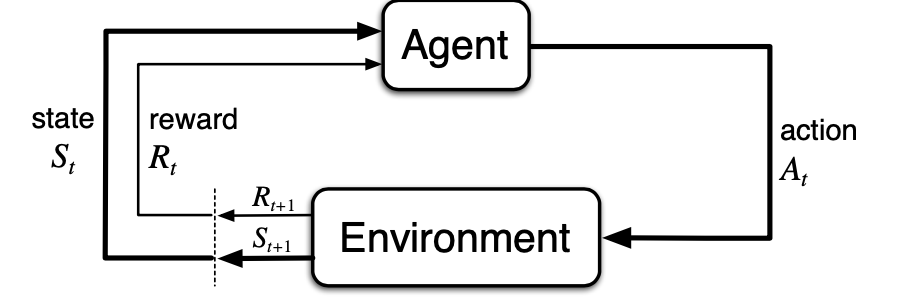
\includegraphics[width=1.0\textwidth]{graphics/markov.png}
    \caption{Ablauf des Markov-Entscheidungsprozess}
    \label{fig:markov_ablauf}
\end{figure}

Der Ablauf wird in \autoref{fig:markov_ablauf} dargestellt und kann laut \cite[S. 636]{castano} als ein \enquote{[...]discrete state-time transition system [...]} beschrieben werden. 
Die zwei Hauptbeteiligten Objekte sind Agent und Umwelt \cite[S. 47ff.]{sutton2018}.
Ein Agent beschreibt eine mit seiner Umwelt interagierende Entität und kann über Software oder Hardware abgebildet werden.
Alle Variablen sind abhängig von diskretisierten Zeitpunkten $t$.
Der Agent erhält zu jedem Zeitpunkt den aktuellen Zustand (engl. state) $s$.
Er kann dann mit der Umwelt z.B. durch Aktoren interagieren, indem er eine Aktion (engl. action) $a \in A_t$ ausführt, wobei die Menge $A_t$ alle Aktionen, die der Agent zum Zeitpunkt $t$ ausführen kann, beschreibt.
Die Wahrscheinlichkeit für den Übergang in den Folgezustand $S_{t+1}$ wird beschrieben durch die Verhaltensstrategie $\pi(a|s_t)$ \cite[S. 58]{sutton2018}.
Für jedes Zustands-Aktions-Paar wird durch eine Belohnungsfunktion eine Belohnung $r_t(s_t, a_t)$ berechnet \cite[S. 638]{castano}.
Ziel ist eine möglichst optimale Abfolge von Aktionen zu ermitteln, um die Summe der Belohnungen zu maximieren.

\section{Begriffe und Eigenschaften von Reinforcement Learning Verfahren}\label{sec:eigenschaften_rl}
Dadurch, dass Reinforcement Learning nicht einen einzelnen Algorithmus beschreibt, sondern ein Paradigma bestehend aus einer Vielzahl von Algorithmen, ist es im Hinblick auf das Ziel dieser Arbeit sinnvoll, die unterscheidenden Merkmale der Verfahren zu betrachten.
Die Begriffe werden als Entscheidungskriterien in \autoref{sec:massnahmen} hinzugezogen, sodass insbesondere im Hinblick auf die Kompabilität mit den in \autoref{sec:def_ethischer_werte} definierten Werten die Wahl eines geeigneten Verfahrens vereinfacht werden kann.
\subsection{Belohnung und Wertfunktion}
Als Reaktion der Umwelt auf eine Aktion des Agenten wird durch eine stochatische Funktion \cite[S. 6]{sutton2018} eine Belohnung zurückgeliefert.
Die Belohnung ist die Grundlage für eine meist unverzügliche Anpassung der Verhaltensstrategie und dient als Indikator über die Güte der ausgeführten Aktion für den jeweiligen Zustand.
Um nachhaltig sinnvolle Entscheidungen zu treffen existiert zusätzlich die Wertfunktion (engl. value function), welche den langfristigen Nutzen von Zuständen approximiert.
So kann beispielsweise ein Zustand einzeln betrachtet stets in einer geringen Belohnung resultieren, langfristig jedoch von gut belohnten Zuständen gefolgt sein.
Die Wertfunktion ordnet diesem Zustand einen hohen Wert zu, die Belohnungsfunktion hingegen einen niedrigen Belohnungswert.

\subsection{Model-freie und Model-basierte Verfahren}
Im Kontext der model-freien und der model-basierten Verfahren bezeichnet das Model die Kenntnis einer Abbildung der Umwelt und dessen Verhalten \cite[S. 7]{sutton2018}.
Das Model der Umwelt wird abgebildet durch eine Zustandsübergangsfunktion \cite[S. 14]{li2018}.
Wird ein model-basiertes Verfahren genutzt, so existiert ein solches Model über die Umwelt und kann genutzt werden, um Vorhersagen über die Auswirkungen von Aktionen zu treffen.
Existiert kein Model muss ein model-freies Verfahren benutzt werden.
Mit Hilfe des Versuchs- und Irrtumsprinzip \cite[S. 7]{sutton2018} versucht der Agent dann, je nach Verfahren ein eigenes Model der Umwelt zu erzeugen.

\subsection{On-Policy und Off-Policy}
On-Policy und Off-Policy beschreiben Lernverfahren, die sich insbesondere durch das Vorgehen bezüglich der Verwendung und Anpassung der Verhaltensstrategie bzw. im Fall des Off-Policy Lernens der Zielstrategie unterscheiden.
Beim Off-Policy Lernen \cite[S. 14]{li2018} wird eine meist statische Vorgehensstrategie (engl. behavior policy) benutzt, welche das Verhalten des Agenten steuert. 
Zusätzlich gibt es eine Zielstrategie (engl. target policy), welche eine möglichst optimale Wertfunktion lernt.
Die Zielstrategie wird basierend auf den erhaltenen Belohnungen für die ausgeführten Aktionen angepasst.
On-Policy-Lernen benutzt nur eine einzelne Verhaltensstrategie, welche ähnlich wie die Zielstrategie des Off-Policy-Lernens angepasst wird, jedoch auch zur Steuerung des Verhaltens des Agenten benutzt wird.
\chapter{Grundlagen der angewandten Ethik und Moral}\label{chap:grundlagen_ethik}
Im Folgenden erfolgt eine Begriffsdefinition und Abgrenzung der Begriffe Ethik und Moral, welche als Grundlage für die in \autoref{sec:def_ethischer_werte} definierten Werte dient.
Im Rahmen dieser Arbeit wird insbesondere die angewandte Ethik betrachtet, da die spätere Konzeption des Vorgehens der Entwicklung einer Reinforcement-Learning-Anwendung stark praxisorientiert erfolgt.

\begin{figure}[h]
    \centering
    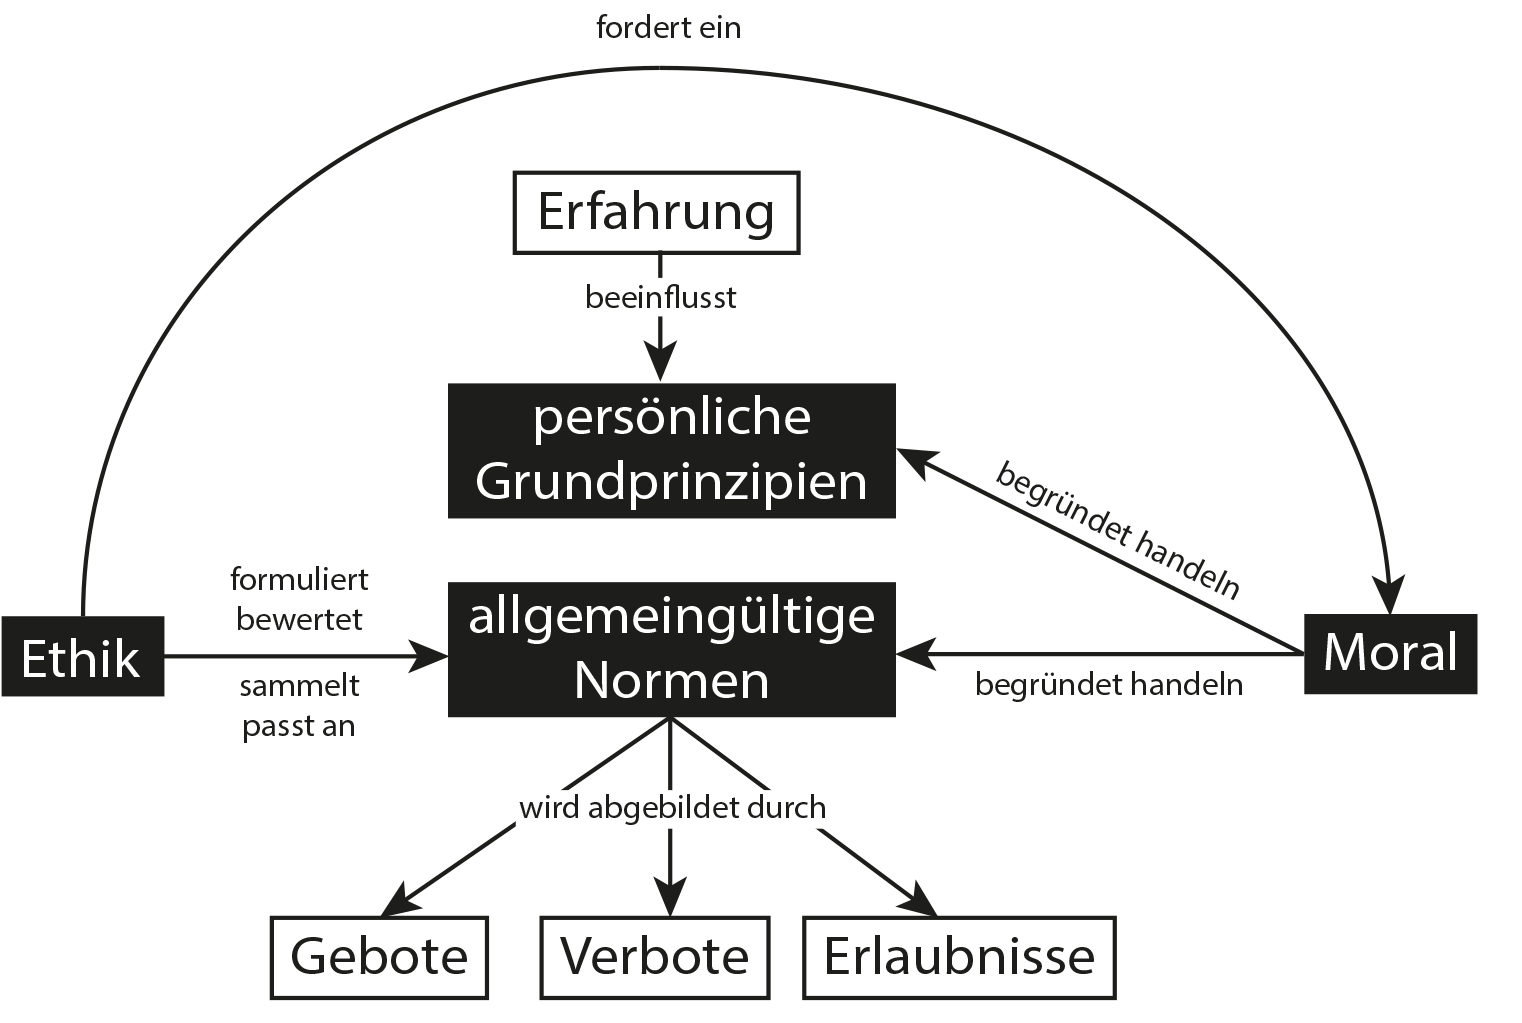
\includegraphics{graphics/ethik_overview.png}
    \caption{Überblick über die Beteiligten Komponenten des moralischen Handelns und dessen Zusammenhang.}
    \label{fig:ethik}
\end{figure}

Sowohl Ethik als auch Moral befassen sich mit Normen, welche in diesem Kontext als \enquote{[...] allgemeingültige Regeln [...]} \cite[S. 10 ff.]{schicha2010} beschrieben werden.
Die angewandte Ethik beschreibt dabei die Formulierung und Bewertung praxisbezogener Normen.
Im Gegensatz zu praxisbezogenen Normen stehen Idealnormen als wünschenswerte aber praktisch nicht umsetzbare Werte.
Als Disziplin der Philosophie fordert die Ethik, wie in \autoref{fig:ethik} abgebildet, nicht nur das Handeln gemäß der Normen ein, sie dient ebenfalls als Sammlung der Gesamtheit aller Normen.
Nicht zuletzt stellt die Ethik auch die Grundlage für die Findung und Anpassung der Normen durch zwischenmenschlichen Diskurs in den Vordergrund.
Auch wenn versucht wird, diesen Prozess rational zu begründen, kann eine Korrektheit nicht, wie etwa in naturwissenschaftlichen Disziplinen, nachgewiesen werden.
Als Wissenschaft ist die Ethik unabhängig von Autoritäten, sondern basiert auf \enquote{[...] Kriterien der Rationalität, der Begründung und der Verallgemeinerungsfähigkeit [...]} \cite[S. 22]{schicha2010}.
Anders verhält sich die Gültigkeit von Normen im Bezug auf den aktuellen Zeitgeist \cite[S. 10]{tannsjo2008}.
Normen können zu jedem Zeitpunkt ihre Gültigkeit verlieren, was jedoch ihre gegenwärtige Gültigkeit und Relevanz nicht einschränkt.
Auf persönlicher Ebene ergeben sich Werte und Normen aus persönlichen Erfahrungen und Interessen \cite[S. 3f]{mcnaughton1988}, was jedoch im Laufe des Lebens von äußeren Einflüssen, wie Religionen und unserer direkten Umwelt beeinflusst wird.
\ab 
Moral bzw. moralisches Handeln ist als praktische Anwendung der, durch die Ethik diskutierten Normen \cite[S. 80]{werkener2017} anzusehen.
Die allgemeingültige Anwendung und Zusicherung von Normen zum Zwecke des moralischen Handelns erfolgt durch Grundprinzipien \cite[S. 11]{schicha2010}, die es ermöglichen auch in vorher unbekannten Situationen gemäß der Normen moralisch zu handeln.
Normen können durch \enquote{[...] Gebote, Verbote und Erlaubnisse [...]} \cite[S. 80]{werkner2017} abgebildet und über die persönliche Moral hinaus formuliert und eingefordert werden.
Sie finden speziell dann Anwendung, wenn das Handeln nicht allein durch die Intuition entschieden werden kann.

\section{Maschinenethik und Einordnung von Reinforcement-Learning-Agenten}
Durch die Komplexität des menschlichen Lebens und Handelns ist es in der angewandten Ethik nur schwer möglich, Normen für jede Situation zu definieren, die allgemeingültig anwendbar sind und dennoch möglichst viele Fälle abbilden.
Deshalb haben sich Bereitsethiken entwickelt, die explizit ein Teilgebiet des menschlichen Lebens abbilden.
Bereichsethiken sind nicht unbedingt auf spezielle Verfahren oder Technologien, sondern viel mehr auf übergeordnete Anwendungen und ethische Fragen eines Systems bezogen.
Ethik ist jedoch kein festgeschriebenes Regelwerk, weswegen im Rahmen dieser Arbeit für die Definition ethischer Werte eine Abstraktion und Generalisierung der verwandten Bereichsethiken und allgemeingültiger Normen erfolgt.
\ab 
Inhaltlich besitzt die Maschinenethik \cite[S. 6]{rath2019} eine größe inhaltliche Nähe zur Thematik des Reinforcement Learning, indem die Anwendungen und ethischen Fragestellungen Überschneidungen aufweisen.
Die Maschinenethik als solche beschreibt zum einen das Verhalten der Menschen im Bezug auf Maschinen und zum anderen, insbesondere im Kontext der lernenden Systeme, das moralische Handeln von Maschinen.
Handeln Agenten z.B. durch die Begrenzung der Fähigkeiten und des Kontextes nicht implizit moralisch, so müssen Normen explizit für die Berücksichtigung in Maschinen  technisch abgebildet werden \cite[S. 34]{bendel2019}.
Dem Agenten soll es dann möglich sein eigenständig in unbekannten Situationen moralisch zu Handeln.
Als Teilgebiet der Ethik ist neben der Umsetzung und Konzeption der Normen auch die Bewertung des Handelns zu betrachten, insbesondere mit dem Ziel das Handeln des Agenten unseren Erwartungen menschlicher Moral zu entsprechen.
Grundlage der Betrachtung explizit ethischer Agenten ist die Frage, ob Maschinen überhaupt moralisch Handeln können.
Laut \cite[S. 41 ff.]{bendel2019} ist die Handlungsfähigkeit als Grundlage des moralischen Handelns an die Fähigkeit zur \enquote{[...] Orientierung an Gründen [...]} \cite[S. 41]{bendel2019} und an die \enquote{[...] Selbstursprünglichkeit [...]}\cite[S. 42]{bendel2019} gekoppelt.
Die Erfüllung dieser Bedingungen ist dabei abhängig von Art und Implementierung eines Systems.
Damit eine Maschine also explizit moralisch handeln kann, muss sie zumindest grundlegend wie ein Mensch handeln.
Die Fähigkeit zur Orientierung an Gründen erfüllen Maschinen, sobald ihr Verhalten an die Erfüllung eines Zieles gebunden oder zumindest dadurch motiviert ist.
Zur Erfüllung der Selbstursprünglichkeit fordert \cite{bendel2019} die Eigenschaften Interaktivität, basale Autonomie und Adaptivität.
Interaktivität und Adaptivität beschreiben dabei die Fähigkeit der Reaktion bzw. der Anpassung des Verhaltens auf äußere Einflüsse und basale Autonomie die Änderung des Zustands ohne äußere Einwirkung.
Erfüllt ein System diese Eigenschaften, so besitzt es zumindest Handlungsfähigkeit und kann, wenn die Gründe für das Handeln einer Moral entsprechen auch moralisch handeln.
\ab 
Im Bezug auf die Thematik des Reinforcement Learning besitzen die daraus entstehenden Agenten eine Orientierung an Gründen, indem die Belohnungsfunktion und das daraus resultierende Ziel die Belohnung zu maximieren das Verhalten beeinflussen.
Zur Erfüllung der Selbstursprünglichkeit müssen zudem Interaktivität, basale Autonomie und Adaptivität betrachtet werden.
Reinforcement-Learning-Agenten können im Sinne der Interaktivität auf äußere Einflüsse reagieren und das eigene Verhalten gemäß der Adaptivität ebenfalls anpassen.
Indem die Agenten einen eigenen Antrieb haben, auch ohne äußere Einflüsse Zustände zu verändern ist auch die basale Autonomie vorhanden.
Dadurch lässt sich darauf schließen, dass Reinforcement-Learning-Agenten zumindest ein gewisses Maß an Handlungsfähigkeit besitzen.
Damit die Agenten nun auch explizit moralisch handeln können, muss die Grundlage des Handelns auf Normen basieren.
Insbesondere in der in \autoref{sec:massnahmen} vorgestellten Maßnahmen zur Entwicklung von ethischen Reinforcement-Learning-Agenten wird die Umsetzung des moralischen Handelns der Agenten auf die in \autoref{sec:def_ethischer_werte} definierten Normen bzw. Werten bezogen.

\chapter{Regionale Zusicherung des ethischen Umgangs mit künstlicher Intelligenz}\label{chap:standards}
Im Folgenden werden Mittel zur Zusicherung ethischen Umgangs mit Anwendungen der künstlichen Intelligenz beispielhaft auf internationaler Ebene, sowie für die Regionen Europa, USA und Asien betrachtet.
Die Zusicherung erfolgt aktuell meist durch Standards und Normen, wobei spezielle Vorgaben für Reinforcement Learning zum Zeitpunkt der Recherche nicht auffindbar sind.
Deshalb wird die Betrachtung auf das Obergebiet der künstlichen Intelligenz ausgeweitet, da die meisten Vorgaben so weit gefasst sind, dass sie ihre Gültigkeit auch für den Teilbereich des Reinforcement Learning behalten.
Eine Betrachtung dieser regionalen Zusicherung ist aus mehreren Gründen interessant.
Die frühzeitige Beachtung der Standards ist insbesondere für die spätere technische Konzeption sinnvoll, da die Vorgaben möglicherweise in der Zukunft als Vorlage für Gesetze dienen können.
Eine Auseinandersetzung mit Standards und Normen signalisiert Anwendern ein Interesse des Herausgebers an ethischen Fragestellungen.
Die Werte sind zudem abhängig von den jeweiligen Rechts- und Kulturräumen.
Die Vorgaben können die dahinterliegenden Wertmaßstäbe, sowie den Stellenwert der Thematik im jeweiligen Raum aufzeigen.

\section{International}\label{sec:international}
Auf internationaler Ebene werden Standards durch die International Organization for Standardization \cite{isoabout} (kurz ISO) entwickelt.
Die ISO besteht aus aus 164 länderspezifisischen Standardisierungseinrichtungen, welche unabhängig von den einzelnen Regierungen sind.
So ist beispielsweise in Deutschland die jeweilige Standardisierungseinrichtung das Deutsche Institut für Normung \cite{din} (kurz DIN), in der USA das American National Standards Institute \cite{ansi} (kurz ANSI) und in China die Standardization Administration China \cite{sac} (kurz SAC).
Ziel ist die Konsolidierung lokaler Standards und damit die Schaffung von Standards auf internationaler Ebene, um möglichst alle Dienste und Produkte \enquote{safe, reliable and of good quality} \cite{iso_benefits} zu gestalten.
Um das zu erreichen sind die Mitglieder in technische Komitees unterteilt, welche die tatsächlichen Standards entwickeln.
Jedem Komitee wird ein Themenbereich zugewiesen, welcher dann Standards entwickelt, diskutiert und später aktualisiert.
\ab 
Da der Prozess der Etablierung von Standards langwierig ist, werden explizit Normen betrachtet, die auf die Oberthematik der Ethik in IT-Systemen allgemein bezogen sind.
Bestehende Normen, wie die ISO-Norm 13482:2014 für private Roboter und die ISO 10218:2012 \cite[S. 50]{wittpahl2019} für industriell eingesetzte Roboter geben Normen für einen Anwendungsbereich des Reinforcement Learning vor, gehen allerdings nicht auf die Technologie explizit ein.
Eine speziellere Betrachtung der Thematik des maschinellen Lernens erfolgt durch das Subkomitee ISO/IEC JTC 1/SC 42.
Zu den hier vorgeschlagenen Normen gehören \cite{iso_sc42}:
\begin{itemize}
    \item \textbf{ISO/IEC CD 22989} \cite{iso22989}: Definition grundlegender Konzepte und Begriffe.
    \item \textbf{ISO/IEC CD 23053} \cite{iso23053}: Definition eines Frameworks zur Nutzung von maschinellen Lernens.
    \item \textbf{ISO/IEC AWI 23894} \cite{iso23894}: Risikomanagement für Künstliche Intelligenz.
    \item \textbf{ISO/IEC AWI TR 24368} \cite{iso24368}: Ethische und soziale Bedenken.
\end{itemize}
Die meisten der Normen des Subkomitees sind allerdings zum aktuellen Zeitpunkt erst in der Konzeptionsphase und müssen noch diskutiert, geprüft und veröffentlicht werden, bevor sie in Kraft treten.
Insgesamt liefert die ISO einen wichtigen Beitrag zur Erstellung weltweit gemeinsamer Standards.
Die Normen sind nicht rechtsbindend, werden aber teilweise als Grundlage für Gesetze genutzt und bieten die Möglichkeit für Herausgeber entsprechender Systemen die Einhaltung dieser Standards nachzuweisen.
\section{Europa}\label{sec:europa}
In Europa gibt es neben nationalen Vereinigungen, wie Bitkom \cite{bitkom} oder der Plattform Lernende Systeme \cite{pls} auch übernationale Vereinigungen, wie Claire \cite{claire}, AI4People \cite{ai4people} oder der HEG-KI \cite{smuha}.
Die Vereinigungen verstehen sich zum Teil als Dachverbände und Vertreter teilnehmender Unternehmen oder als Gruppen, welche sich aus Experten der Forschung und Wirtschaft zusammensetzen.
Sie unterscheiden sich durch die Zusammensetzung der Mitglieder, sowie durch den Aufbau und die Ziele.
Im Fall von AI4People bestehen die Mitglieder z.B. aus internationalen Unternehmen, wie Facebook, Intel und Microsoft.
Im Gegensatz dazu besteht beispielsweise die Plattform Lernende Systeme etwa zum gleichen Anteil aus Vertretern der Wirtschaft und der Wissenschaft und ist in sieben Arbeitsgruppen zu unterschiedlichen Domänen des Oberthemas lernende Systeme aufgeteilt.
Dort gibt es z.B. explizit eine Arbeitsgruppe zum Thema Ethik von lernenden Systemen \cite{plsa}.

\subsection*{Ethik-Leitlinien der HEG-KI}
Im Folgenden sollen exemplarisch die Ethik-Leitlinien der Hochrangingen Expertengruppe für Künstliche Intelligenz (kurz HEG-KI) betrachtet werden.
Die Expertengruppe wird offiziell von der europäischen Kommission eingesetzt und ist an alle Beteiligten gerichtet.
Also vom Bürger über den Entwickler bis zu Unternehmen und Behörden.
Es wird Wert auf den europäischen Ursprung der entwickelten Inhalte gelegt, um Unabhängigkeit zu wahren.
Inhaltliche Grundlage ist die Verbesserung der Lebensqualität der Bürger, die Umsetzung von Nachhaltigkeit und die Minimierung möglicher Risiken.
Das Handeln soll gemäß der europäischen Werte \enquote{Menschenrechte, Demokratie und Rechtsstaatlichkeit} \cite[S. 6]{smuha} erfolgen.
Die Pfeiler dieser Werte sind laut der HEG-KI Rechtmäßigkeit, Ethik und Robustheit.
Ziel ist die Definition einer vertrauenswürdigen künstlichen Intelligenz.
Dafür werden Grundsätze und Bewertungskriterien zur \enquote{Entwicklung, Einführung und Nutzung von KI-Systemen} \cite[S. 3]{smuha} aufgezeigt.
Das Vorgehen soll den gesamten Prozess der Entwicklung begleiten, möglichst unabhängig sein und sieht einen dauerhaften Abgleich mit den Anforderungen vor.
Es ist eingeteilt in Fundamente, Verwirklichung und Bewertung.
Die Zusicherung und Umsetzung der Maßnahmen ist unterteilt in technische- und nichttechnische Maßnahmen, wodurch möglichst alle Beteiligten miteinbezogen werden soll.
\ab 
Ziel des Dokumentes ist die Standardisierung für die Entwicklung und Nutzung ethischer KI-Anwendungen.
Es soll Vertrauen innerhalb der Gesellschaft schaffen, indem grundlegende Konzepte erklärt und jegliche Entscheidungen fachlich begründet werden.
Allen Beteiligten soll ein Vorgehen aufgezeigt werden, mit dem ethische KI-Anwendungen strukturiert werden können.
Auch wenn die Leitlinien zunächst nicht bindend sind, ist die Definition sinnvoll.
So haben Herausgeber durch die Richtlinien frühzeitig die Möglichkeit, dem Gesetzgeber, sowie Anwendern ein Bemühen bei der Umsetzung ethischer KI-Anwendungen nachzuweisen.
\section{USA}\label{sec:usa}
In der USA gibt es das IEEE \cite{ieee} als weltweit größter Fachverband mit über 420\,000 Mitgliedern aus technischen Berufen in 160 Ländern \cite[S. 287]{chatila2019}.
Ziel ist die Förderung von Innovation und Technologie zum Wohle des Menschen zu lenken.
Deshalb hat das IEEE in \citetitle{chatila2019} diverse Aspekte des ethischen Softwaredesign betrachtet.
\ab 
Neben dem allgemeinen Vorgehen werden Grundprinzipien, rechtliche Grundlagen, sowie Tipps zur Implementierung aufgelistet.
Zu den Grundprinzipien zählen z.B. die Einhaltung und Beachtung der Menschenrechte, sowie die physische und emotionale Unversehrtheit des Menschen, die Nachvollziehbarkeit, Effektivität und ein hinreichendes Maß an Kompetenz der Entwickler.
Inhaltlich werden explizit Entwickler angesprochen.
Ziel des Dokumentes ist die Verbesserung des menschlichen Lebens durch KI-gestützte Maschinen, die explizit ethische Richtlinien befolgen und so den Menschen dienen \cite[S. 6]{chatila2019}.
Die allgemeine Beschreibung stellt dabei den Anfang einer Reihe von tatsächlichen Standards in der IEEE-Gruppe \enquote{P7000 - Model Process for Addressing Ethical Concerns During System Design}\cite[S. 283]{chatila2019} \cite{emelc-wg} dar.
\section{Asien}\label{sec:asien}
Durch ein großes Engagement asiatischer Länder im Bereich der Förderung und Forschung \cite[S. 46]{tsinghuauniversity} Künstlicher Intelligenz werden im Folgenden Maßnahmen asiatischer Länder betrachtet.
So haben exemplarisch dafür im Jahr 2017 23 \% aller KI-Unternehmen ihren Sitz in China gehabt \cite[S. 142]{ding}.
China selbst hat mehrere Pläne veröffentlicht \cite[S. 8]{ding}, um das Vorgehen für die Zukunft in unterschiedlichen Teilbereichen der künstlichen Intelligenz zu fördern, um bis 2030 das weltweite Zentrum der Forschung und Anwendung von KI zu sein.
Deshalb wird im Folgenden betrachtet, wie ethische Kriterien asiatischer Länder zugesichert werden soll.
\ab 
China, Singapur, Australien, Malaysia und Indien haben bereits Institutionen gebildet \cite{mit2019}, um ethische KI-Fragen zu diskutieren.
So hat Indien beispielsweise mit \#AIforAll \cite{nitiaayog2018} die nationale Strategie veröffentlicht, in der insbesondere Fokus auf den Nutzen für die Gesellschaft und ethischen Umgang gesetzt wird.
Lediglich Japan, Südkorea und Taiwan legen aktuell wenig bis keine Priorität auf ethische Bedenken von KI Anwendungen \cite{mit2019}, auch wenn einige dieser Länder in der Vergangenheit schon nicht rechtlich verbindliche Standards diskutiert haben.
Viele Universitäten engagieren sich dabei für internationale Lösungen und arbeiten eng mit ihren jeweiligen Regierungen zusammen.
Ziel ist der Aufbau von Vertrauen in die bestehenden Menschen- und Datenschutzrechte, ohne dabei Fortschritt und Innovation zu behindern.
Nahezu alle Länder sind an der Diskussion beteiligt und sehen Potenzial in der Technologie als zukünftigen Wirtschaftszweig.
Dennoch werden beispielsweise von China Anwendungen, wie die flächendeckende Nutzung von Gesichtserkennung \cite{mozur2018} genutzt, welche in der Form nicht vereinbar mit unseren europäischen Werten sind.
\chapter{Diskussion} \label{chap:diskussion}
Im Folgenden wird zunächst der Kontext dieser Arbeit auf Grund der Komplexität der Thematik inhaltlich abgegrenzt.
Anschließend werden Anwendungsgebiete des Reinforcement Learning aufgezeigt, um die Relevanz und mögliche Bedenken aufzuzeigen.
Es werden zudem verwandte Arbeiten betrachtet und inhaltlich mit dieser Arbeit verglichen.
Zuletzt werden Herausforderungen für die Entwicklung des Vorgehensplans betrachtet, welche als Anforderungen und spätere Bewertungsgrundlage dienen.

\section{Abgrenzung}\label{sec:abgrenzung}
Wenn die Rede von einem autonomen System ist, so wird im Kontext dieser Arbeit insbesondere ein Reinforcement Learning gestütztes System betrachtet.
Da Reinforcement-Learning-Systeme allerdings Überschneidungen mit anderen KI-Systemen aufweisen, sind die Aussagen teilweise auch auf diese übertragbar.
Die Kernproblematik ist meist ähnlich, unterscheidet sich allerdings insbesondere durch die Lösungsansätze.
Ziel der Arbeit ist die technischen Konzeption von ethischen Werten für Reinforcement-Learning-Anwendungen.
Zu beachten ist dabei, dass der technische Ansatz im Rahmen dieser Arbeit nur ein Mittel ist, um die ethischen Werte umzusetzen.
Nicht beachtet werden explizit technische Eigenschaften, wie beispielsweise Integrität, Interoperabilität oder Wartbarkeit, auch wenn diese möglicherweise implizit durch die Zusicherung der ethischen Werte abgedeckt werden.
\ab 
Das Oberthema der künstlichen Intelligenz ist sehr umfangreich, weswegen eine inhaltliche Abgrenzung sinnvoll ist.
Zunächst wird als Technologie ausschließlich Reinforcement Learning betrachtet. 
Die im Rahmen der Arbeit betrachteten Agenten sind beschränkt auf die Interaktion mit der Umwelt.
Eine Interaktion mit anderen Agenten in einer Multiagentenumgebung wird nicht betrachtet.
Ebenso werden starke, also domänenübergreifende oder selbstverbessernde Agenten nicht betrachtet, da es zum Zeitpunkt der Arbeit im Rahmen der Recherche neben \cite{hall2007} keine aktuellen Belege für den praktische Einsatz bzw. die Möglichkeit zur Nutzung gibt.
Inhaltlich werden sowohl Reinforcement-Learning-Agenten in Form von Expertensystemen mit indirektem Einfluss, wie auch Agenten mit direktem Einfluss in Form von Robotern o.Ä. betrachtet, da beide Agententypen Anwendung finden und eine enge inhaltliche Nähe aufweisen.
In \autoref{sec:stand_der_technik} werden teilweise andere Arbeiten aufgezeigt, die abgegrenzte Themen behandeln.
\section{Anwendungsgebiete und Stand der Technik}\label{sec:stand_der_technik}
Im Folgenden wird der Stand der Technik in zweierlei Hinsicht betrachtet.
So wird zunächst ein Überblick über Möglichkeiten und Anwendungsgebiete des Reinforcement Learning aufgezeigt und anschließend Ansätze der Umsetzung von Ethik in Reinforcement-Learning-Anwendungen betrachtet und mit der Konzeption des Entwicklungsprozess ethischer Agenten im Rahmen dieser Arbeit verglichen.
Dadurch wird die Relevanz der Thematik, sowie Unterschiede zu bestehenden Arbeiten aufgezeigt.

\subsection{Anwendungsgebiete}
Reinforcement Learning wird speziell in Anwendungsbereichen eingesetzt, in denen der Agent autonom in fremden Situationen agieren muss.
Im Folgenden werden als Anwendungsbereiche exemplarisch autonomes Fahren, autonome Waffensysteme und Einsatzgebiete im Gesundheitswesen betrachtet.
Innerhalb dieser Anwendungsgebiete wird Reinforcement Learning zum einen als Aktor in Form von Robotik eingesetzt, aber auch als unterstütztende Expertensysteme.

\subsubsection{Autonomes Fahren}
Fahrzeuge mit Fahrassistenzsystemen oder Teilautonomie sind schon jetzt ein relevantes Thema innerhalb der Automobilindustrie bei Unternehmen, wie beispielsweise Daimler, Google, Volkswagen oder Tesla, mit einem Gesamtmarktwert von über fünf Milliarden US-Dollar im Jahr 2018 \cite{businesswire2019}.
Bestehende Arbeiten, wie \cite{arvind2019} oder \cite{niu2009} beschreiben die Implementierung von Teilkomponenten des autonomen Fahrens in virtuellen Umgebungen, indem Aufgaben, wie die Kollisionsvermeidung gesondert betrachtet werden.
\cite{you2019} betrachtet als Teilproblem die intelligente Verkehrssteuerung, in dem das Verhalten autonomer Fahrzeuge im Bezug auf Verkehrsfluss und Verbrauchseffizienz optimiert wird.
\cite{yu} beschreibt einen Einsatz des autonomen Fahrens, indem durch Deep-Q-Learning die Steuerung eines virtuellen Fahrzeuges erlernt und der Einfluss unterschiedlicher Belohnungsfunktionen auf den Fahrstil beobachtet wird.
In \cite{sallab2017} wird als Grundlage für die Entwicklung ein Frameworks für autonomes Fahrens vorgestellt, welches durch Kombination von Deep Reinforcement Learning und Rekurrenten Neuronalen Netzen (engl. recurrent neural network) grundlegende Funktionen, wie Steuerung, Abbildung von Umgebungen und die Interaktion mit anderen Fahrzeugen implementiert.
Das Training autonomer Fahrzeuge ist durch die Natur der Fahrzeuge nur unter großem Kostenaufwand und mit beträchtlichem Risiko durchzuführen.
So wird in \cite{pan2017} eine Möglichkeit vorgestellt, um simulierte Umgebungen mit Hilfe von realen Bildern abzubilden, wodurch die realitätsnähe simulierter Agenten verbessert werden soll.

\subsubsection{Autonome Waffensysteme}
Reinforcement Learning in autonomen Waffensystemen wird insbesondere bei der Entwicklung und dem Einsatz unbemannter Luftfahrzeuge (engl. unmanned aerial vehicles, kurz UAV) in Form von Quadrocoptern verwendet, da diese durch ihre Bauform und die daraus resultierende Flugstabilität diverse Vorteile gegenüber anderen Bauformen bieten \cite{bou-ammar2010}.
Ähnlich wie bei Anwendungen des autonomen Fahrens werden auch bei autonomen Waffensystemen Teilprobleme betrachtet.
So beschreibt \cite{bou-ammar2010} in \cite{bou-ammar2010} die Nutzung verschiedener Reinforcement-Learning-Verfahren für die Steuerung von UAVs.
Zusätzlich zur tatsächlichen Steuerung werden z.B. in \cite{zhang2015} Möglichkeiten zur Identifikation einer möglichst optimalen Route für mehrere UAVs unter Betrachtung der Routenlänge und der Risikobewertung durch andere Agenten aufgezeigt. 
\cite{koch2019} beschreibt den Einsatz von Reinforcement Learning für die Höhensteuerung im Hinblick auf Stabilität und Kontrollmöglichkeiten als weitere Teilkomponente für die Steuerung von UAVs.
Neben der eigentlichen Fortbewegung von autonomen Waffensystemen findet Reinforcement Learning auch Einsatz in Abwehrsystemen.
So wird in \cite{xiao2018} beschrieben, wie die Verbindungsqualität von UAVs durch Reinforcement Learning gegen Störsignale gesichert werden kann, indem die Kommunikation und mögliche Angriffe im vorhinein simuliert und das Verhalten dementsprechend angepasst wird.

\subsubsection{Gesundheitswesen}
Im Gesundheitswesen ist der Einsatz autonomer Systeme wünschenswert, um medizinisches Personal zu entlasten, die Fehlerquote zu reduzieren und die begrenzte Menge an spezialisierten Experten zu skalieren.
Neben dem Einsatz von Robotik im Gesundheitswesen ist die Anwendung von Expertensystemen sinnvoll, um die Gefährdung von Patienten zu limitieren.
Durch Nutzung von Expertensystemen muss die Durchführung der vorgeschlagenen Entscheidungen von Menschen getroffen werden, wodurch Entscheidungen frühzeitig hinterfragt werden können.
So wird beispielsweise in \cite{liu2017} und in \cite{mulcahylevy2018} Reinforcement Learning genutzt, um einen möglichst optimalen Behandlungsplan zu entwickeln und an mögliche Änderungen während der Behandlung anzupassen.
In \cite{richter2019} wird eine simulierte Operationsumgebung vorgestellt, welche gemäß bestehender Standards implementiert ist und mit entsprechender Schnittstelle genutzt werden kann.
Ziel ist dabei, die Entwicklung weiterer Umgebungen zu motivieren und so die Vergleichbarkeit neuer Algorithmen zu gewährleisten.
Zur Optimierung von Robotern im Gesundheitswesen wird in \cite{woodworth} eine Möglichkeit zur Anpassung des Verhaltens gemäß der Vorgaben der Nutzen durch Inverse Reinforcement Learning vorgeschlagen.
So können Roboter durch Beobachtung des Nutzers generalisieren und entsprechend der Erwartungen handeln.

\subsection{Verwandte Arbeiten}
Im Folgenden sollen Arbeiten aufgezeigt werden, die inhaltlich ebenfalls die Betrachtung ethischer Bedenken bei der Umsetzung von KI-Anwendungen, im Speziellen von Reinforcement-Learning-Anwendungen behandeln.
Dadurch kann für die spätere Konzeption eine Grundlage der Entwicklung geschaffen werden und Alleinstellungsmerkmale dieser Arbeit herausgestellt werden.
\ab 
Inhaltlich verwandt sind zunächst die in \autoref{chap:standards} vorgestellten Beispiele zur Zusicherung ethischer Richtlinien.
Darin werden beispielsweise in \cite{smuha} Grundlagen der Technologie eingeführt und Vorstellungen bezüglich Ethik-Richtlinien von der Europäischen Union oder in \cite{chatila2019} von der IEEE aufgezeigt.
Dabei sind alle Maßnahmen bezogen auf künstliche Intelligenz als Oberthema.
Im Vergleich zu dieser Arbeit wird der Fokus nicht speziell auf Reinforcement Learning, sondern höchstens auf potenzielle Anwendungen gelegt.
Weiterhin werden nicht explizit technische Maßnahmen vorgeschlagen, sondern eher Richtlinien, die bei Umsetzung individuell erarbeitet werden müssen.
\ab 
In \cite{cointe} wird moralisches Handeln in Multiagenten-Systemen betrachtet.
Dabei wird in \cite{cointe} ein Model entwickelt, welches das eigene und das Verhalten der anderen Agenten in der Umgebung ethisch bewertet.
Ähnlich zum Vorgehen im Rahmen dieser Arbeit basiert die ethische Bewertung auf Grundlage moralphilosophischer Konzepte.
Unterschiedlich ist allerdings die Vorgehensweise.
So werden in \cite{cointe} die Normen und moralischen Prinzipien technisch abgebildet, um das Handeln gemäß der eigenen Einschätzung zu beschränken.
Die Normen müssen zunächst definiert und bei der Anwendung regelbasiert abgefragt werden.
Daraus ergeben sich zwei Probleme.
Zum einen müssen die Normen formalisiert werden, was insbesondere bei komplexen Situationen nicht trivial bzw. nicht realistisch umsetzbar ist.
Zum anderen wird das moralische Handeln nicht als Teil des Lernens miteinbezogen, wodurch der Agent kein eigenes Rechtsbewusstsein erhält.
Anders als bei dieser Arbeit werden zudem Multiagenten-Umgebungen betrachtet und ein regelbasiertes Vorgehen vorgeschlagen.
So wird im Rahmen dieser Arbeit ein allgemeines organisatorisches und technisches Vorgehen und nicht eine einzelne Maßnahme beschrieben.
\ab 
In \cite{noothigattu} wird ein Agent erstellt, der mit Hilfe von Inverse Reinforcement Learning ethischen Normen folgen soll.
Im Gegensatz zu \citeauthor{cointe} werden die Normen nicht regelbasiert vor der Entscheidungsfindung abgefragt, sondern durch Beobachtung von Experten gelernt.
Neben einer Verhaltensstrategie zur Belohnungsmaximierung existiert dann eine zweite Verhaltensstrategie, die gemäß des beobachten Verhaltens moralisch handelt.
Je nach Situation wird dann nachvollziehbar entschieden, welche Aktion und damit welche Verhaltensstrategie sinnvoller ist.
Dieser Ansatz in \cite{noothigattu} lässt, ähnlich wie in \cite{cointe}, jegliche organisatorische Maßnahmen außen vor.
Ebenso kann das Verfahren durch die Wahl der jeweiligen Verfahrensstrategie lediglich entscheiden, ob effizient oder ethisch gehandelt wird.
Im Rahmen dieser Arbeit ist das Ziel, den Agent möglichst zu jedem Zeitpunkt moralisch handeln zu lassen und organisatorische und technische Maßnahmen zu vereinen.
\section{Herausforderungen}\label{sec:Herausforderungen}
Im Folgenden werden Herausforderungen betrachtet, die bei der Konzeption technischer Maßnahmen zur Erstellung eines Vorgehensplans für die Entwicklung ethischen Reinforcement Learnings auftreten können.

\subsection{Subjektivität moralischen Handelns}
Agenten können die Werte der Entwickler widerspiegeln, indem unterschiedliche Arten der Beeinflussung (engl. bias) \cite{sengupta2018} bewusst oder unbewusst in die Datenerhebung und die spätere Entwicklung einfließen.
Beispiele dafür sind z.B. Stereotypisierung oder eine einseitige Auswertung und Anpassung bezüglich der Klassenverteilung.
Dadurch, dass die Entwicklung von Reinforcement-Learning-Anwendungen oft in größeren, heterogenen Teams geschieht, sollten Maßnahmen ergriffen werden, damit die Beteiligten ein, mit den geforderten Werten an die Anwendung, kompatibles Wertesystem besitzen.
Ebenso sollten Maßnahmen ergriffen werden, um Verzerrungen zu identifizieren und diese je nach Grad der Abweichung als Fehler zu betrachten und Möglichkeiten der Beseitigung dieser Verzerrung in Betracht gezogen werden.

\subsection{Problem der Formalisierung}
Moralisches Handeln ist abhängig von der jeweiligen Situation.
Einfache Entscheidungen werden meist intuitiv getroffen und können dementsprechend nur schwer formalisiert werden.
Im Gegensatz dazu stehen Situationen, in denen durch Komplexität und Uneindeutigkeit moralischer Prinzipien Dilemma \cite[S. 300]{moll2003} entstehen.
In Diesem Fall ist die Entscheidungsfindung hochgradig dynamisch und abhängig von einer analytischen Denkweise, in der versucht wird, mögliche Folgen abzuwägen.
Es stellt sich neben der Problematik der Formalisierbarkeit der intuitiv-emotionalen Entscheidungen die Problematik bezüglich der technischen Abbildung des komplexen Prozesses im Falle eines moralischen Dilemmas.
Neben der Formalisierung der Entscheidungsprozesse müssen diese Werte und Normen nach denen moralisches Handeln erfolgt formalisiert werden, um in Agenten technisch abgebildet werden zu können.

\subsection{Mangelnde Zertifizierung}
Sicherheitskritische Anwendungen können Vertrauen gewinnen, indem die Korrektheit der Implementierung und Prozesse durch vertrauenswürdige Institutionen geprüft und anschließend bestätigt wird.
Projektebezogene Prozesse und Grundlagenalgorithmen können durch gängige Institutionen und Normen zertifiziert werden.
Durch die Aktualität und insbesondere die Komplexität von Reinforcement Learning konnte im Rahmen der Recherche jedoch keine explizite Möglichkeit zur Zertifizierung speziell von Reinforcement Learning Systemen im Gesamten identifiziert werden.
Zwar gibt es Ansätze z.B. vom Fraunhofer-Institut für Intelligente Analyse- und Informationssysteme \cite{cremers} für die Zertifizierung von KI-Anwendungen, allerdings wird zum Zeitpunkt der Arbeit lediglich ein Prüfkatalog als Grundlage der späteren Zertifizierung entwickelt.
Umso wichtiger ist es dann, Vertrauen aufzubauen und Korrektheit transparent und nachvollziehbar selbständig nachzuweisen.

\subsection{Innovation, Fortschritt und Adaption}
Insbesondere auf internationaler Ebene versuchen alle Beteiligten einen Vorsprung im Bereich künstlicher Intelligenz zu erlangen.
Treiber dieses internationalen Wettlaufs sind dabei Innovation und Fortschritt.
Dem gegenüber steht das Potenzial des Reinforcement Learning Wohl und Würde des Menschen zu gefährden.
Die Definition expliziter ethischer Werte und die daraus resultierenden Maßnahmen sollen die Wahrung fördern und die Relevanz der Einhaltung eben dieser aufzeigen.
Es gilt, blinden Fortschritt zu verhindern und stattdessen frühzeitig ethische Werte zu diskutieren, sowie Maßnahmen zur Zusicherung zu identifizieren.
Optimalerweise unterstützt die Betrachtung ethischer Werte die Adaption in der Gesellschaft, Wirtschaft und Politik, indem Vertrauen aufgebaut wird.
Um dies zu unterstützen bedarf es neben dem Einfordern der Gesellschaft der Berücksichtigung ethischer Bedenken und gesetzlichen Regelungen seitens der Politik, technische und organisatorische Maßnahmen möglichst kompatibel mit bestehenden Prozessen und Technologien zu definieren und aufzuzeigen, inwiefern ethisches Verhalten wirtschaftlich sinnvoll sein kann.
\ab 
Neben dem Bestreben nach Fortschritt stehen allerdings auch Bedenken der Gesellschaft.
Eine breite Adaption innerhalb der Gesellschaft ist Grundlage der Beteiligung von Unternehmen am Fortschritt zwecks wirtschaftlichen Interesses.
Die Adaption wird z.B. durch die Diffusionstheorie \cite[S. 513 ff.]{karnowski2013} beschrieben.
Auf persönlicher Ebene entsteht die Entscheidung zur Adaption als Folge gewisser Grundvorrausetzungen, dem Wissensstand und der persönlichen Abwägung bezüglich der Nutzung.
Zu den Grundvoraussetzungen gehören Erfahrungen mit ähnlichen Technologien, die Existenz von Probleme, die die Technologie löst, das Maß an Innovation und der persönliche Kontext.
Durch Hinzunahme des persönlichen Verständnisses der Technologie wird abgewägt, wie groß der Nutzen im Verhältnis zur Komplexität der Adaption und wie kompatibel es mit der persönlichen Situation ist.
Um eine Adaption zu fördern müssen diverse Herausforderungen betrachtet werden.
Dazu gehört die digitale Kluft \cite{rogers2016} als Wissenlücke bezüglich digitaler Technologien zwischen gesellschaftlichen Gruppen.
Ebenso müssen Fähigkeiten, Limitierungen der Technologie transparent gemacht und relevante Nutzungskontexte für die Gesellschaft identifiziert werden.
Zusätzlich muss ein Mindestkenntnisstand etabliert, sowie die Komplexität der Anwendungen auf ein Maß reduziert werden, um die Technologie attraktiv zu gestalten.
\ab 
Grundlage der persönlichen Entscheidung zur Adaption ist die Kenntnis über den tatsächlichen Einsatz der Technologie. 
Zum Zeitpunkt der Arbeit besteht allerdings keine Kennzeichnungspflicht bezüglich des Einsatzes von KI-Technologien.
Reinforcement Learning ist dabei oft nicht eine eigenständige Anwendung, sondern Teilkomponente in bestehenden Systemen.
Die Entscheidung bezüglich der Adaption ist dabei nur dann relevant, wenn der Nutzer auch einen tatsächlichen Einfluss auf die Nutzung haben kann.
So haben beispielsweise Menschen in Kriegsgebieten keinen Einfluss auf den Einsatz autonomer Waffensysteme.
Umso wichtiger ist dann die Schaffung gesetzlicher Rahmenbedingungen, bezüglich des Einsatzes von Reinforcement Learning und der Beachtung gewisser ethischer Werte und der Umsetzung geeigneter Maßnahmen zur Zusicherung dieser Werte.

\chapter{Konzeption}\label{chap:konzeption}
Im Folgenden werden  zunächst ethische Werte basierend auf den in \autoref{chap:grundlagen_ethik} eingeführten Grundlagen der Ethik und den in \autoref{chap:standards} betrachteten Maßnahmen internationaler Institutionen begründet.
Anschließend wird ein Vorgehensplan vorgestellt, der technische und organisatorische Maßnahmen enthält, mit denen entlang eines üblichen Softwareprojektablaufs gemäß \cite[S. 64]{broy2013} die Zusicherung der ethischen Werte umgesetzt werden kann.

\section{Definition ethischer Werte}\label{sec:def_ethischer_werte}
Die Wahl ethischer Grundwerte für die Entwicklung und Anwendung von Reinforcement-Learning-Anwendungen wird im Folgenden auf Grundlage ethischer Prinzipien, sowie bestehender Standards und Normen begründet.
Ziel ist eine Konsolidierung bestehender Ansätze für die in \autoref{sec:massnahmen} vorgestellte Konzeptionierung eines praktischen Maßnahmekataloges.
Die Werte sollen dabei klar verständlich und möglichst allgemeingültig sein.
Überkulturelle Grundlage ist im Allgemeinen die Achtung der Menschenrechte \cite{vereintenationen1948}.
Oberstes Ziel sollte die Zusicherung und Wahrung eben dieser sein.
Zusätzlich macht es Sinn, ethische Werte zuzusischern, um neben der Unversehrtheit von Wohl und Würde des Menschen, auch Vertrauen in die Technologie aufzubauen.
Die Wahl der Werte wird in den einzelnen Unterkapiteln näher erläutert, basiert jedoch stark auf den in \autoref{chap:standards} vorgestellten Normen und Standards der einzelnen Regionen.
Um nicht von einzelnen Verfahren innerhalb der Technologie und Domäne abhängig zu sein, sind die Werte möglichst allgemein gehalten.
Bei der Definition auftretende Fragen sollen im Rahmen dieser Arbeit nicht unbedingt behandelt werden, sondern dienen viel mehr zu Veranschaulichung der Relevanz und der Problematik dieser Werte.
\subsection{Nachvollziehbarkeit und Erklärbarkeit}\label{sub:nachvollziehbarkeit}
Die ethische Entscheidungsfindung besteht laut \cite[S. 4]{tannsjo2018} aus zwei Komponenten.
Zum einen aus der Anwendung gelernter moralischer Prinzipien und zum anderen aus der Hinzunahme möglichst aller relevanter Informationen.
Dieser Prozess der ethischen Entscheidungsfindung ist insbesondere bei der Bewertung eines Agenten relevant.
Ein Agent soll gemäß unserer menschlichen Werte handeln und muss deshalb auch gemäß dieser bewertet werden.
Nachvollziehbarkeit bezieht sich dabei zum einen auf die Kenntnis über vergangene und möglicherweise die Absicht der Ausführung zukünftiger Aktionen und zum anderen auf die Fähigkeiten und Limitierungen des Systems, sowie auf den Entstehungsprozess.
Insbesondere für Entscheidungsprozesse von domänenfremden Verantwortungsträgern müssen Güte und Entstehungsprozess nachvollziehbar sein, dadurch dass Weiterentwicklung und Optimierung darauf basieren.
Erklärbarkeit fordert zusätzlich, dass Entscheidungen nicht nur nachvollzogen, sondern begründet werden können.
Die Werte Nachvollziehbarkeit und Erklärbarkeit bieten die Grundlage für die Zusicherung der folgenden zwei Werte.
So kann das in \autoref{sub:vertrauen} geforderte Vertrauen nur dann aufgebaut werden, wenn durch das System ein Verständnis seitens der verantwortlichen Personen, insbesondere des Entwicklers über das Handeln entsteht und Personen im Anwendungskontext auf Grund der Erklärbarkeit ihr Handeln ggfs. anpassen und das des Agenten einschätzen können.
Die Frage der in \autoref{sub:verantwortung} beschriebenen Verantwortung basiert zudem auf der Grundlage, dass alle verantwortwortlichen Personen das Verhalten des Agenten kennen, nachvollziehen können und der Prozess der Entscheidungsfindung mit den persönlichen Werten übereinstimmt.

\subsection{Vertrauen durch Kalkulierbarkeit und Zuverlässigkeit}\label{sub:vertrauen}
Vertrauen ist insbesondere bei der Adaption ein wichtiger Treiber und damit Grundlage des Fortschrittes der hier betrachteten Technologien.
Vertrauen entsteht dann, wenn alle beteiligten Parteien eine gemeinsame \enquote{[...] Basis geteilter Normen, Werte und positiver Zukunftserwartungen [...]}\cite[S. 61]{gilberta} besitzen.
Es ermöglicht Kalkulierbarkeit unabhängig von rechtlichen Verpflichtungen \cite[S. 61 ff.]{gilberta}.
Vertrauen kann in diesem Anwendungsbereich in der Regel nicht in einzelne Personen aufgebaut werden, da bei komplexen Softwaresystemen oft große Teams zum Einsatz kommen und das Produkt somit Ergebnis der Zusammenarbeit vieler ist.
Deshalb muss das Unternehmen als ganzes ein Systemvertrauen aufbauen, indem Anwender auf die Prinzipien des Unternehmens vertrauen können.
Zuverlässigkeit in Form von Korrektheit und Robustheit in unbekannten Situationen können helfen Vertrauen langfristig aufzubauen \cite[S. 13]{avizienis2004}.
Die Anforderungen des Systems, sowie das tatsächliche Handeln müssen zum Aufbau von Vertrauen mit den Erwartungen übereinstimmen und können nur erfüllt werden, wenn das System kalkulierbar handelt.

\subsection{Verantwortung und Schuld}\label{sub:verantwortung}
Sobald Agenten Einfluss auf Menschen nehmen können, muss geklärt werden, wer Verantwortung für die Folgen des Handelns eines Agenten und damit die Schuld im Fehlerfall trägt \cite[S. 88]{heckman1998}.
Verantwortung ist dabei die notwendige Bedingungen, um tatsächlich Schuld zuzuweisen \cite[S. 75]{duttge2009}.
Die Verantwortung wird zum einen von der Umwelt gefordert \cite[S. 1]{hoffrage2019} und zum anderen von Innen durch das persönliche Gewissen der Verantwortlichen erbracht.
Durch korrekte Dokumentation kann für einzelne Teile eines Systems zwar die Frage der verantwortlichen Person ermittelt werden, gerade bei selbstlernenden Systemen sind die verursachenden Verhaltensweisen jedoch nicht explizit implementiert, sondern entstehen möglicherweise als unerwünschte Randeffekte.
Deshalb ist die Frage der Verantwortung und Schuld insbesondere bei selbstlernenden Systemen nicht trivial und sollte im Laufe des Produktlebenszyklus betrachtet werden.
Eine Bestrafung im Sinne der Schuld trägt bei Maschinen keine Wirkung.
Die Frage der Schuld betriftt also die Verantwortlichen.
Laut \cite[S. 76]{duttge2009} \enquote{[...] kann man niemanden für die Verletzung einer Norm zur Rechenschaft ziehen, die er gar nicht einhalten konnte [...]}.
Im Bezug zu selbstlernenden und insbesondere autonomen Systemen stellt sich also die Frage, ob ein Verantwortlicher die Verletzung der Norm beeinflussen kann.
So ist beispielsweise ein Kriegseinsatz nur dann rechtmäßig, wenn die Verantwortung für mögliche Tode eindeutig geklärt ist.
Zu klären bleibt dann, inwiefern ein Einsatz gerechtfertigt ist, wenn z.B. ein autonomes Waffensystem zwar weniger Fehler macht als Menschen, die Schuldfrage jedoch nicht eindeutig geklärt werden kann.

\section{Vorgehensplan zur Zusicherung ethischer Werte}\label{sec:massnahmen}
Die Umsetzung der in \autoref{sec:def_ethischer_werte} definierten ethischen Werte soll entlang eines üblichen Softwarelebenszyklus \cite[S. 64]{broy2013} erfolgen, da die ethischen Probleme in allen Phasen Beachtung finden müssen.

\begin{figure}[ht]
    \centering
    \frame{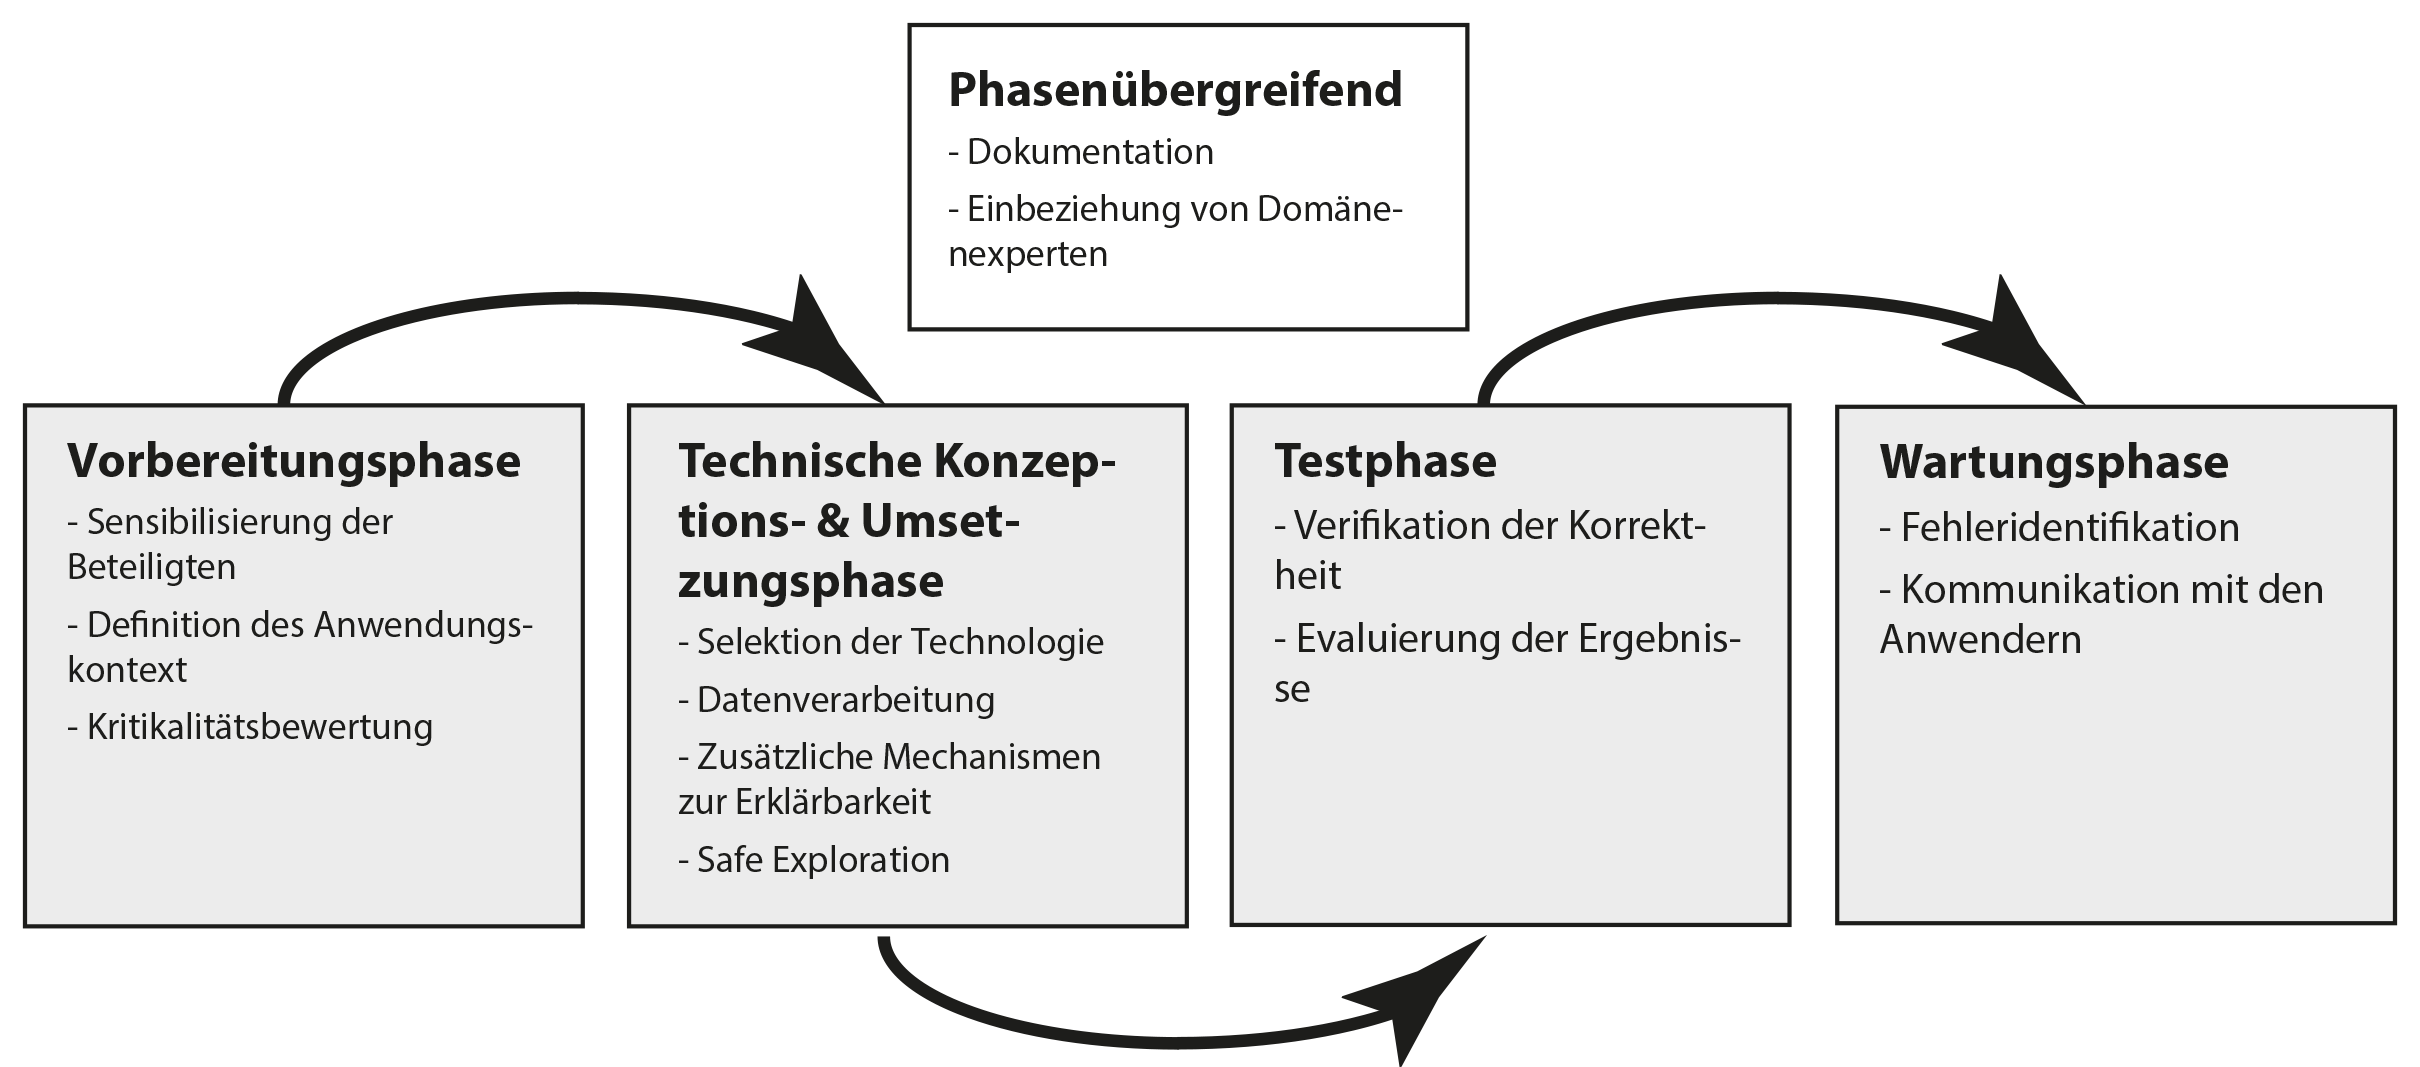
\includegraphics[width=\textwidth]{graphics/guidelines.png}}
    \caption{Phasen und jeweilige Maßnahmen der Zusicherung ethischer Werte.}
    \label{fig:guidelines}
\end{figure}

Die in \autoref{fig:guidelines} skizzierten Maßnahmen werden im Folgenden hinsichtlich der ethischen Werte begründet.
Das Vorgehen soll kompatibel mit den meisten Vorgehensmodellen sein, indem die Phasen so allgemein gefasst sind, dass sie nahezu in allen Vorgehensmodellen in irgendeiner Form vorkommen.
Die Phasen können parallel zu den jeweiligen Phasen im Vorgehensmodell durchgeführt werden.
Viele Maßnahmen behalten ihre Gültigkeit über die jeweilige Phase hinweg, sollten jedoch spätestens ab der vorkommenden Phase beachtet werden.
Es wird kein spezieller Fokus auf einzelne Domänen gesetzt.
Stattdessen werden allgemeine Hinweise und Möglichkeiten aufgelistet, wodurch eigene Maßnahmen abgeleitet werden können.
Viele der Maßnahmen beziehen sich im Speziellen auf sicherheitskritische Anwendungen.
Innerhalb der Phasen wird zunächst das Ziel der jeweiligen Phase erläutert und anschließend technische und organisatorische Maßnahmen vorgestellt.
Ziel dieses Vorgehens ist die Definition von Leitlinien, die mit den in \autoref{sec:def_ethischer_werte} vorgestellten Werten kompatibel sind und in bestehende Prozesse integriert werden können.
\ab 
Vorweg werden Maßnahmen eingeführt, die phasenübergreifend gültig sind und ggfs. innerhalb der einzelnen Phasen spezieller betrachtet werden.
So ist Dokumentation in jeder Phase ein wichtiges Mittel, um das Verhalten nachvollziehen zu können, Vertrauen durch Transparenz aufzubauen und Verantwortung zuordnen zu können.
Welche Informationen dabei in den einzelnen Phasen relevant sind, wird an passender Stelle jeweils beschrieben.
Alle dokumentierten Informationen sollten langfristig und in einem menschlich lesbaren Format gespeichert werden.
Optimalerweise wird die Dokumentation ähnlich wie eine Lizenzangabe mit der Software bzw. dem Agenten ausgeliefert.
In dem Fall muss die Dokumentation möglichst klar und dem Wissensniveau des Anwenders entsprechend formuliert sein.
Neben einer ausführlichen Dokumentation ist phasenübergreifend eine Miteinbeziehung von Domänenexperten sinnvoll \cite[S. 12 ff.]{gottesman2018}.
Domänenexperten können schon während des Entstehungsprozesses Einfluss auf die inhaltliche Korrektheit ausüben.
Um ethisches Handeln zuzusichern, kann zudem z.B. in allen Entwicklungsschritten eine explizite Aufforderung der Übereinstimmung der formulierten Werte und der moralischen Prinzipien der Mitarbeiter gefordert und die Zustimmung oder mögliche Mängel dokumentiert werden.
Ebenso fordert die Miteinbeziehung von Domänenexperten implizit Erklärbarkeit und Nachvollziehbarkeit ein, indem zum Verständnis der Experten Aktionen des Agenten nichttechnisch aufbereitet werden müssen.
Domänenexperten können zudem genutzt werden, um die Realitätsnähe simulierter Umgebungen und des Aktionsraumes zu validieren.
Reinforcement Learning tendiert durch Fehler, wie Reward Hacking dazu, nicht gängige Methoden zur Belohnungsmaximierung zu finden.
Um dies zu vermeiden können Domänenexperten das Verhalten der Agenten einordnen und so unübliche frühzeitig Methoden identifizieren.
\subsection{Vorbereitungsphase}\label{sub:vorbereitungsphase}
In der Vorbereitsphase sollen zunächst grundlegende Informationen gesammelt und der Anwendungskontext klar abgegrenzt werden.
Dafür werden zusätzlich organisatorische Anforderungen aufgezeigt, um die ethischen Werte zu berücksichtigen.
Es soll eine klare Definition des Einsatzzweckes, der Absichten und der Anforderungen definiert werden und so eine solide Grundlage für die späteren Phasen entstehen.

\subsubsection{Sensibilisierung der Beteiligten}
Zur Umsetzung der Maßnahmen müssen alle beteiligten Personen für das Thema Ethik sensibilisiert sein.
Dadurch können bereits frühzeitig personelle Probleme erkannt und Lösungen gefunden werden.
Die Motivation für die Durchsetzung ethischer Maßnahmen kann sowohl von außen, also extrinsisch, als auch von den Personen selber, also intrinsisch, erfolgen \cite{baum2017}.
Intrinsische Motivation kann nur begrenzt beeinflusst werden und ist hauptsächlich vom Wertesystem des Einzelnen, aber auch von seiner Umgebung abhängig.
Einfluss kann darauf durch extrinsische Maßnahmen ausgeübt werden, indem beispielsweise die sozialen Normen innerhalb des Unternehmens Ethik als Kernthema enthalten und durch unabhängige Instanzen überprüft und eingefordert werden.
Um Teil der Gemeinschaft zu sein kann sich so beim Einzelnen eine intrinsische Motivation entwickeln, die mit den Unternehmensnormen übereinstimmt.
Auf der anderen Seiten kann eine extrinsische Motivation durch das Unternehmen oder durch die Politik und Gesellschaft eingefordert werden.
Maßnahmen dazu sind beispielsweise Gesetze, welche den Einsatz bestimmter Technologien verbieten.
Ebenso können Vorgaben des Unternehmens und daraus potenziell resultierende Strafen oder umgekehrt Belohnungen bei Einhaltung eine Möglichkeit sein, um ethisch korrektes Handeln zu motivieren.
\subsubsection{Definition des Anwendungskontext}
Im Folgenden werden Maßnahmen und Fragestellungen betrachtet, die zur klaren Definition des Einsatzzweckes, der Absichten und Anforderungen relevant sind.
Die Maßnahmen sollten bereits bei der Erhebung der Anforderungen beachtet werden.
\\\\
\\\\
\begin{qanda}
    \Q Welche Aufgaben soll das System haben? 
    \A Eine realistische und präzise Definition der Aufgaben und Ziele des Systeme bietet die Grundlage der Entwicklung.
    Gemäß \enquote{AI is not magic} \cite[S. 13]{gottesman2018} sind hier bereits Schwächen und Grenzen der zu nutzenden Technologie zu beachten.
    
    \Q In welchem Kontext soll das System eingesetzt werden?
    \A Zu beachten sind Rechts- und Kulturräume, öffentliche und private Einsatzzwecke, sowie Einzel- und Multiagentenumgebungen und die Einbettung in andere IT-Systeme.
    
    \Q Welche Limitierungen soll das System haben und welchen Werten soll es folgen?
    \A KI-gestütze Systeme sollten einen klaren Anwendungskontext besitzen und dementsprechend auch Limitierungen ihrer Funktionalität.
    Die klare Definition und öffentliche Kommunikation dieser Limitierungen kann helfen, Vertrauen aufzubauen.
    Ebenso sollte frühzeitig entschieden werden, welchen Werten das System folgen soll, da die Abbildung der Werte in gesamten Produktlebenszyklus beachtet werden muss.
    
    \Q Soll der Agent explizit oder implizit ethisch handeln?
    \A Implizit ethische Agenten sind durch ihren Anwendungskontext nicht in der Lage unethisch zu handeln. 
    In dem Fall muss ein Fokus darauf gelegt werden, den Agenten auf genau diesen Kontext zu begrenzen.
    Ist dies nicht der Fall, müssen für den Agenten explizit Maßnahmen ergriffen werden, um die ethischen Werte umzusetzen.
    Diese Maßnahmen werden in den Folgenden Phasen vorgestellt.
    
    \Q Wie erfolgt der Einfluss auf die Umgebung, insbesondere auf Menschen?
    \A Agenten können z.B. als Expertensystemen einen indirekte Einfluss auf ihre Umwelt besitzen, indem die Entscheidungen von anderen Systemen ausgeführt werden müssen.
    Im Gegensatz dazu besitzen Agenten mit direktem Einfluss auf die Umwelt Aktoren, um selbständig mit der Umwelt zu interagieren.
    Die Entscheidung, um welche Art von Agent es sich im Bezug auf den Einfluss auf die Umwelt handelt, ist essentiell für die spätere Beachtung der Maßnahmen und hat einen großen Einfluss auf die Kritikalitätsbewertung.
\end{qanda}

Als Ergebnis entsteht neben einer notwendigen Grundlage für den späteren Entwicklungsprozess eine Kritikalitätsbewertung.
Die Kritikalitätsbewertung gibt Aussage darüber, welche Mitarbeiter am Projekt beteiligt sein dürfen, wie der Umgang mit den dazugehörigen Daten aussehen muss, welche Verfahren zu wählen sind, was maximale Eingriffs- und Anpassungszeiten im Fehlerfall sind und in welchem Maße die Prozesse geprüft und zertifiziert werden müssen.
Die in den späteren Phasen beschriebenen Maßnahmen können eine Hilfestellung geben diese Fragen zu beantworten.


\subsection{Technische Konzeptions- und Umsetzungsphase}\label{sub:umsetzungsphase}
Im Folgenden werden Maßnahmen zum Softwaredesign basierend auf den in \autoref{sub:vorbereitungsphase} erhobenen Anforderungen vorgestellt.
Zusätzlich werden Technologien zur praktischen Umsetzung der in \autoref{sec:def_ethischer_werte} definierten ethischen Werte im Kontext einer Reinforcement-Learning-Anwendung betrachtet.
Dafür werden mögliche technische Probleme betrachtet, die mit der Umsetzung der ethischen Werte kollidieren und Maßnahmen aufgezeigt, die diesen Problemen entgegenwirken.

\subsubsection{Selektion der Technologie}
Die Wahl des Reinforcement-Learning-Verfahrens sollte durch die Beachtung ethischer Werte nicht auf wenige Einzelne beschränkt werden, sondern bestehende so angepasst und genutzt werden, dass sie den Anforderungen entsprechen können.
Um Vertrauen zu gewinnen ist die Nutzung standardisierter Implementierungen von Grundlagenalgorithmen sinnvoll.
Zum aktuellen Zeitpunkt konnten im Rahmen der Recherche keine Normen identifiziert werden, nach denen Reinforcement-Learning-Systeme zertifiziert werden können.
Als Alternative zur Zertifizierung des Gesamtsystems ist es sinnvoll, Standardimplementationen einzelner Algorithmen zu benutzen.
So bietet beispielsweise das Forschungsinstitut OpenAI \cite{openai} eine Sammlung an Standardimplementierungen \cite{dhariwal2017}.
Diese sind zwar nicht offiziell zertifiziert, werden aber durch OpenAI und durch die Open-Source-Gemeinschaft gepflegt und getestet.
Auch wenn die Nutzung dieser Algorithmen Potenzial hat, eine bessere Vergleichbarkeit zu gewährleisten und die Korrektheit zu erhöhen, sollte ein intensiver Fokus auf die Testphase gelegt werden und so ein eigener Nachweis der Korrektheit erbracht werden.
\ab
Es existiert eine Vielzahl an Reinforcement-Learning-Verfahren mit unterschiedlichen Eigenschaften, die in \autoref{sec:eigenschaften_rl} beschrieben wurden.
Allgemeingültige Empfehlungen bezüglich eines einzelnen Verfahren sind nicht sinnvoll, da die Technologie sich stetig verändert und die Wahl des Verfahrens stark vom Anwendungskontext abhängig ist. 
Die Entscheidung sollte auf Grundlage der Abwägung der Stärken und Schwächen der einzelnen Verfahren und Eigenschaften getroffen werden.
Bei der Wahl des Verfahren ist insbesondere die Komplexität der Umwelt zu beachten.
Agiert der Agent ausschließlich in einer begrenzten Domäne, ist die Wahl eines model-basierten Verfahrens sinnvoll.
So kann eine Repräsentation der Umwelt erzeugt werden, womit die Folgen von Aktionen im Vorhinein approximiert werden können.
Neben der Unterscheidung zwischen model-basierten und model-freien Verfahren ist zu entscheiden, ob gemäß On-Policy oder Off-Policy gelernt wird.
Off-Policy-Learning tendiert eher zur Entdeckung (engl. exploration) \cite[S. 24]{herrmann} neuer Aktionsfolgen, wohingegen On-Policy-Learning eher in Richtung der bestehenden Verhaltensstrategie tendiert.
Insbesondere bei sicherheitskritischen Anwendungen ist ein starker Fokus auf Entdeckung, zumindest in einer realen Umgebung, nicht wünschenswert.

\subsubsection{Datenverarbeitung}
Reinforcement Learning ist abhängig von den gesammelten Daten der Umwelt.
Sind die Daten inkorrekt oder manipuliert, kann die Korrektheit und damit die Gesamtgüte des Systems kompromittiert werden.
Auch wenn Reinforcement Learning ein Online-Learning-Verfahren ist, werden Daten möglicherweise transformiert, indem beispielsweise der Zustandsraum zeitlich diskretisiert wird.
Ebenso kann von der Sammlung dieser Daten, insbesondere der Entscheidungen des Agenten profitiert werden.
Um die Korrektheit der Daten sicherzustellen empfiehlt sich die Sicherstellung der Datenherkunft (engl. data provenance) \cite[S. 3]{olufowobi2017}.
Data Provenance beschreibt die Dokumentation der Geschichte des Ursprungs und der Transformation der Daten.
Durch ein entsprechendes Datenmodell wird ermöglicht nachzuvollziehen, wie die Daten entstanden sind und wie sie transformiert werden.
Zusätzlich kann durch Data Provenance Poisoning als Angriff abgemildert werden, indem Veränderungen der Daten nachvollzogen werden können.
Poisoning beschreibt einen Angriff, bei dem eine gezielte Veränderung der Umgebung vorgenommen wird, wodurch das Verhalten beeinflusst wird \cite[S. 103]{baracaldo2017}.
Durch diese Maßnahmen kann konstant die Korrektheit und Neutralität der Daten-Pipeline sichergestellt werden, indem nachvollzogen werden kann, inwiefern die Transformation der Ausgangsdaten den Anforderungen entspricht.
\ab 
Neben der Transformation der Daten sollte auch die Entstehung der Daten betrachtet werden.
Insbesondere in praktischen Anwendungen dienen Sensoren oft als Datenquelle und können Abnutzungserscheinungen erleiden, indem sie verändert oder beschädigt werden \cite[S. 113]{kramer2009}.
Wünschenswert ist deshalb eine regelmäßige automatische und manuelle Überprüfung der Sensorik, wobei zu beachten ist, dass diese Veränderung ggfs. nicht auffällig ist.
In diesem Fall sollte ein Fail-Safe-Mode vorhanden sein, da ein reguläres Abschalten des Systems ebenfalls eine Gefährdung darstellen kann.

\subsubsection{Zusätzliche Mechanismen zur Erklärbarkeit}
Je nach Verfahren weißt Reinforcement Learning ein unterschiedliches Maß an Erklärbarkeit auf.
Wird beispielsweise ein tabulares Verfahren benutzt, so können die eigentlichen Entscheidungen transparent nachvollzogen werfen, dadurch dass die Daten und die Entscheidungsstrategie zu jedem Zeitpunkt bekannt sind.
Bei Verfahren, die künstliche neuronale Netze \cite[S. 187]{sutton2018} nutzen gibt es das Problem der Erklärbarkeit, was bei vielen überwachten Lernverfahren üblich ist, in dem der eigentliche Entscheidungsprozess als Blackbox anzusehen ist.
Durch Algorithmen wie LIME (local interpretable model-agnostic explanations) \cite{ribeiro2016} kann Erklärbarkeit auch bei künstlichen neuronalen Netzen gewährleistet werden.
LIME erstellt ein zusätzliches interpretierbares Model, welches inhaltlich gleich zum eigentlichen Model ist.
Interpretierbare Verfahren, wie Entscheidungsbäume, bieten die Möglichkeit durch nicht abstrakte Attribute eine Visualisierung anzubieten, die es dem Betrachter ermöglicht die Entscheidungsgrundlage nachzuvollziehen.
\ab 
Ein anderer Ansatz für die Zusicherung von Erklärbarkeit von Reinforcement-Learning-Verfahren wird in \cite{sequeira2019} beschrieben.
Ziel des Verfahren ist die Identifikation von \enquote{interestingness elements} \cite[S. 2]{sequeira2019}, also von Elementen, die die Entscheidung durch einen hohen Informationsgehalt beeinflussen.
Um das zu erreichen werden zusätzlich diverse Informationen gesammelt bzw. generiert.
Die Informationen bestehen aus:
\begin{itemize}
    \item Häufigkeit einzelner Beobachtungen $z$ und wie oft daraufhin eine Aktion $a$ ausgeführt wurde.
    \item Häufigkeit und Wahrscheinlichkeit, wie oft eine Beobachtung $z'$ als Folge eines vorhergegangen Entscheidungstupels $(z, a)$ erfolgt ist.
    \item Geschätzter Nutzen des Entscheidungstupels $(z, a)$.
    \item Geschätzter Nutzen $z$ zu beobachten.
\end{itemize}
Die Informationen werden analysiert, um Informationen über relevante Elemente zu erhalten und zu bewerten inwiefern diese zur Entscheidungsfindung beitragen.

\subsubsection{Safe Exploration}
Safe Exploration beschreibt eine Sammlung von Maßnahmen, um einen Agenten auf sichere Art und Weise eine Umgebung erkunden zu lassen.
Eine sicherer Erkundungsprozess ist dann wichtig, wenn der Agent in unbekannten Umgebungen agiert. 
Auch dann sollte der Lernprozess keine Menschen in der Umgebung gefährden.
In \cite[S. 14 ff.]{amodei2016} werden diverse Möglichkeiten vorgeschlagen, um Safe Exploration umzusetzen.

\begin{description}
    \item \qa{Veränderte Optimierung der Verhaltensstrategie}
    Die Verhaltensstrategie soll nicht anhand der Maximierung der Gesamtbelohnung optimiert wird, sondern auch anhand des Verhaltens in selten eintretenden Fällen.
    \item \qa{Simulation der Umwelt}
    Projekte, wie OpenAI Gym \cite{brockman2016} bieten eine standardisierte Schnittstelle zur Erstellung simulierter Umgebungen, wobei viele bekannte Szenarien, wie die Bewegung gewisser Roboter bereits implementiert sind.
    Viele Reinforcement-Learning-Anwendungen folgen einem iterativen Prozess des \enquote{[...] continual cycle of learning and deployment [...]}\cite[S. 15]{amodei2016}.
    Neben der Optimierung des Verfahrens kann es sinnvoll sein auch die Umgebung nach jedem dieser Schritte abhängig von den Resultaten und den daraus resultierenden Probleme zu optimieren.
    Dadurch können Fehler, wie eine zu starke Anpassung oder Reward Hacking, also das Erlernen nicht generalisierbaren Verhaltens für ein spezielles Problem verhindert werden.
    \item \qa{Begrenzung der Umgebung}
    Findet das System zwangszweise Anwendung in einer realen Umwelt, kann es sinnvoll sein diese zu begrenzen.
    Dabei kann die Definition von sicheren Zuständen, insbesondere eines sicheren Startzustandes helfen, Risiken zu minimieren.
    Zusätzlich kann für jede Aktion geprüft werden, ob das Ausführen zur Folge hätte, dass der sichere Zustand verlassen wird.
    \item \qa{Überwachung durch Menschen}
    Die Überwachung des Agenten kann auf unterschiedlichen Arten erfolgen.
    So kann beispielsweise gefordert werden, dass jede Aktion durch einen Menschen freigegeben werden muss, was allerdings bei Echtzeitanwendungen einen starken Einfluss auf die Performanz hat. 
    Eine abgeschwächte Variante dieses Verfahrens ist die Begrenzung des autonomen Handelns auf klar definierte sichere Zustände, wobei beim Verlassen dieser Zustände eine Zusicherung eines Menschen erfordert wird.
    Beide Aktionen sind ggfs. sehr langsam, da je nach Modellierung Aktionen sehr schnell erfolgen können.
    Trotzdem sichert die menschliche Überwachung die Forderung von \cite{hellbardt1996} zu, dass Entscheidungen über die Ziele der Agenten beim Anwender belassen sein sollten.
    Zusätzlich bietet der menschliche Einfluss ein erhöhtes Maß an Sicherheit gegenüber unerwünschter Handlungen, sowie eine klarere Definition der Verantwortung.
\end{description}

\subsubsection{Sonstige Maßnahmen}
Folgende Maßnahmen haben eine zu hohe inhaltliche Distanz zu den anderen Maßnahmen oder einen zu geringen Einfluss auf die Umsetzung der ethischen Werte und sollen deshalb der Vollständigkeit halber lediglich aufgezählt werden.
\begin{itemize}
    \item Klare Kennzeichnung der Absicht des Agenten durch Statusanzeigen o.Ä.
    \item Apprenticeship Learning \cite{abbeel2004} als Möglichkeit unter menschlicher Überwachung zu lernen.
    \item Reward Shaping bzw. Reward Engineering \cite{karampatziakis2019} kann helfen das System zu optimieren. Überlicherweise wird als Optimierungsmetrik der Verhaltensstrategie ein direktes Feedback der Umgebung bzw. des Nutzers verwendet. Die Identifikation von indirektem Feedback sollte analysiert werden und möglicherweise zusätzlich zum direkten Feedback genutzt werden.
    \item Verzerrungen durch Daten und Entwickler beachten \cite{thomson2001a}.
    Die Daten sind stark von der Modellierung der Umwelt und der Einschätzung und Wissensstand der Entwickler abhängig und damit auch anfällig für die Verzerrung des Verhaltens durch die persönlichen Werte der Entwickler.
\end{itemize}

\subsection{Testphase}\label{sub:testphase}
Ziel der Testphase ist die Überprüfung der Korrektheit der vorhergangenen Implementierung gemäß Funktionalität, Robustheit und der Erfüllung der Anforderungen.
Um tatsächlich Vertrauen in die Korrektheit des Systems zu gewinnen müssen Evaluierungsprozess und Dokumentation transparent und nachvollziehbar sein.
Dafür werden im Folgenden zum einen die Prozesse der Verifikation, sowie der Evaluation von Reinforcement-Learning-Systemen betrachtet.

\subsubsection{Verifikation der Korrektheit}
Gängige Verifikationsverfahren für Softwaresysteme, wie Modelprüfung (engl. model-checking) sind beim Reinforcement Learning nicht ohne Anpassung nutzbar \cite[S. 12 ff.]{vanwesel2017}, da das System durch den stetigen Lernprozess verändert wird.
Model-Checking kann z.B. dann benutzt werden, wenn nur ein einzelner Zeitpunkt des Systems betrachtet wird.
Grundlage der Verifikation ist die klare Erhebung der Anforderungen und Limitierungen in \autoref{sub:vorbereitungsphase}, welche als Spezifikation für die Verifikation benutzt werden.
Zu unterscheiden ist zwischen Offline-Verifikation, welches Verifikationsverfahren beschreibt, die zu festen Zeitpunkten genutzt werden können und Online-Verifikation, welches Verifikationsverfahren beschreibt, die in dynamischen Systemen benutzt werden können.
\ab 
Obwohl Reinforcement Learning ein Online-Lernverfahren beschreibt, können einige Spezifikation auch offline verifiziert werden.
So können bei model-basierten Verfahren Markov-Entscheidungsprozesse über Werkzeuge, wie PRISM (Probalistic Symbolic Model Checker) \cite{prism} automatisch verifiziert werden.
Bei model-freien Verfahren muss das Model erst gelernt werden und kann dann, analog zu den model-basierten Verfahren getestet werden.
Neben des Markov-Entscheidungsprozess können bei Reinforcement-Learning-Anwendungen die eingesetzten Grundlagenalgorithmen mit regulären Offline-Verfahren getestet werden.
Zusätzlich lassen sich Aussagekraft und Güte der Trainingsdaten in Form von Eigenschaften, wie der Verteilung oder Unabhängigkeit durch statistische Verfahren testen.
\ab
Durch die sich ständig verändernde Natur eines Online-Lernverfahrens ist Online-Verifizierung bzw. \enquote{runtime verification} \cite[S. 16]{vanwesel2017} rechen- und speicherintensiv.
Das grundlegende Vorgehen bei Online Verification basiert auf der Annahme, dass, wenn die Spezifikation vor Beginn des Lernens und bei jeder Änderung erfüllt ist, die Spezifikation als Ganze erfüllt ist.
Geprüft werden dann die Zustands-Aktionspaare hinsichtlich ihrer Übereinstimmung mit der Spezifikation.
In der Spezifikation müssen neben den Anforderungen auch die Limitierungen abgebildet sein und durch das Verifikationsverfahren geprüft und zugesichert werden.
\ab 
Auch wenn das Gesamtsystem als solches nicht mit nur einem Verfahren verifiziert werden kann, so kann durch die Kombination mehrerer Verfahren und die Verifikation einzelner Teilkomponenten eine Verbesserung von Korrektheit und Robustheit und damit der Zuverlässigkeit erzielt werden.
Die Definition der Spezifikation muss allgemein genug definiert sein, sodass möglichst viele Sachverhalte abgedeckt sind, aber auch so speziell, dass die Eigenheiten des Systems und des Anwendungskontexts abgebildet werden.

\subsubsection{Evaluierung der Ergebnisse}
Ziel der Evaluierung ist die Bewertung der Güte des Modells anhand nachvollziehbarer Metriken.
Die Metriken erbringen den Nachweis über die Zuverlässigkeit und ermöglichen einen sachlichen Vergleich mit anderen Systemen.
Aussagekräftige Metriken erlauben zudem die Schaffung realistischer Erwartungen \cite[S. 13]{gottesman2018}.
Eine Einordnung der Güte eines Systems sollte in Relation zu anderen Systemen und insbesondere zur menschlichen Leistung im Anwendungskontext gesetzt werden \cite{deswarte2019}.
Um die Nachvollziehbarkeit der Ergebnisse und des Evaluierungsprozesses zu gewährleisten sollte eine kontrollierte Umgebung genutzt werden.
Der Aufbau einer simulierten oder realen Umgebung sollte durch Seeds zur Zufallszahlengenerierung und andere Parameter nachvollzogen werden können.
Ebenso sollten weitere Evaluationskriterien, wie die Wahl der Hyperparameter, sowie Implementationen der Algorithmen und je nach Verfahren die Netzwerkarchitektur dokumentiert werden.
\ab 
Zusätzlich zur tatsächlichen Messverfahren zur Evaluation des Systems sollte die Verhaltensstrategie des Agenten \cite[S. 13 f]{gottesman2018} analysiert werden.
Insbesondere durch Hinzunahme von Domänenexperten können Abweichungen des gewünschten Verhaltens identifiziert werden.
Die technische Umsetzung der Nachvollziehbarkeit hilft dem Domänenexperten einen tieferen Einblick in das Verhalten des Agenten zu erlangen und so möglicherweise Randeffekte zu bewerten und Ursachen dafür zu identifizieren.
Eine solche Analyse ist nicht nur bei der endgültigen Verhaltensstrategie, sondern auch nach jedem Iterationsschritt der Entwicklung sinnvoll, um frühzeitig Optimierungspotenzial oder Fehlverhalten zu identifizieren.
\subsection{Wartungsphase}\label{sub:wartungsphase}
Grundlage dieser Phase ist das fertige System, welches im realen Anwendungsfall eingesetzt wird.
Zur Wartung im Speziellen von Reinforcement-Learning-Systemen sind in Folge der intensiven Literaturrecherche im Rahmen dieser Arbeit nahezu keine Informationen entsprungen.
Deshalb werden im Folgenden allgemeine Maßnahmen zur Wartung von Software-Systemen beschrieben und auf Grundlage meiner persönlichen Meinung auf die Thematik des maschinellen Lernens bzw. des Reinforcement Learning bezogen.
Die Wartungsphase bietet das Potenzial, langfristig Vertrauen aufzubauen und nachhaltig zu stärken.
In dieser Phase behalten insbesondere die Umsetzungsphase in \autoref{sub:umsetzungsphase} und die Testphase in \autoref{sub:testphase} ihre Relevanz.
Insbesondere die Testphase sollte bei der Umsetzung von Fehlerverbesserungen beachtet werden, um neue Fehler zu vermeiden.
Die hier beschriebenen Maßnahmen sollten stets mit dem Ziel ausgeführt werden, dass in den Phasen bis zum Endprodukt aufgebaute Vertrauen zu stärken und im Fall der Weiterentwicklung und Einführung neuer Funktionen das Vertrauen in die Neuerungen herzustellen.
Als Dokumentation ist in der Wartungsphase insbesondere ein Änderungsprotokoll (engl. changelog) sinnvoll, um dem Anwender nachvollziehbar Nachweise über Änderungen und deren Inhalt zu geben.
Ziel ist die Wahrung bzw. die Zusicherung eines möglichst nachhaltig zuverlässigen Zustand des Systems.
\ab 
Fehler können auch durch ausgiebiges Testen nicht gänzlich ausgeschlossen werden \cite[S. 533]{balzert2011}.
Insbesondere bei Systemen mit hoher Kritikalitätsbewertung ist eine Wartung im Sinne der Fehlerausbesserung bis zur endgültigen Außerbetriebnahme sinnvoll.
Ist dies nicht der Fall, so sollte der Anwender klar über die Dauer des Wartungszeitraumes und über ein Ablaufen dieses Zeitraumes frühzeitig informiert werden.
Die Wartung des Systems sollte dessen Funktionalität nicht verändern, sondern Zuverlässigkeit und Korrektheit zusichern.
Grundlage der Fehlerausbesserung ist die Fehleridentifikation, welche durch die Logdatenanalyse, eine aktive Fehlersuche durch Entwickler aus Softwaresicht, von Domänenexperten durch Verhaltensanalyse oder durch Rückmeldung der Anwender erfolgen kann.
Die Kommunikation mit den Anwendern ist insbesondere deshalb sinnvoll, weil die Vielzahl der Anwendungskontexte und Aufgabengebiete Situationen hervorruft, die in der Entwicklung- und Testphase nicht abgedeckt werden können.
Neben den typischen Softwarefehlern bietet Reinforcement Learning Potenzial zusätzlicher Fehlerquellen, die in \cite[S. 3]{amodei2016} beschrieben werden.
Dazu gehört das unerwünschte Verhalten, bei dem sich durch die stetige Veränderung des System das Verhalten so ändert, dass es nicht mehr den vorher definierten Anforderungen entspricht.
Eine weitere Fehlerform ist die unnatürliche Belohnungsmaximierung (engl. reward hacking).
Reinforcement-Learning-Agenten können unnatürliches Verhalten entwickeln, welches zwar Aktionen wählt, die die Belohnung maximieren, jedoch nicht gängigen Methoden entspricht und damit potenziell gefährlich sein kann.
\ab
Werden Fehler identifiziert gilt es, diese gemäß der Kritikalität einzuordnen und dementsprechend zu handeln.
Insbesondere bei Fehlern in Anwendungen mit hoher Kritikalität sollten Anwender und Betroffene informiert und das System ggfs. bis zur Nachbesserung stillgelegt werden.
\chapter{Evaluation}\label{chap:evaluation}
Im Folgenden erfolgt eine Evaluation der Ergebnisse dieser Arbeit hinsichtlich der in \autoref{chap:einleitung} gestellten Fragestellungen und der in \autoref{sec:Herausforderungen} definierten Herausforderungen für die Konzeption.
Zur Gewährleistung der Übersichtlichkeit werden die jeweiligen Bewertungsgrundlagen angegeben, inhaltlich passend zusammengefasst und anschließend diskutiert, inwiefern diese erfüllt werden.

\section{Formalisierung ethischer Werte}
Die Formulierung ethischer Werte ist die Grundlage des moralischen Handelns von Reinforcement-Learning-Agenten und der eigentlichen Konzeption organisatorischer und technischer Maßnahmen zur Zusicherung eben dieser.
Die Forderung nach der Formalisierung ethischer Werte besteht dabei aus zwei Problemen.
So sind ethische Werte abhängig vom sozialen Umfeld und persönlichen Erfahrungen und sind damit subjektiv.
Zum anderen werden moralische Entscheidungen in der Regel intuitiv bzw. im Fall moralischer Dilemma hoch komplex und damit schwer formalisierbar getroffen.
\ab 
Um diese Probleme zu lösen wurde deshalb zur Schaffung des inhaltlichen Bezuges zunächst Grundlagen der angewandten Ethik und Moral vermittelt und die Frage danach, ob moralisches Handeln von Agenten überhaupt möglich ist betrachtet.
Zusätzlich wurden Vorschläge und Begründungen bezüglich der Zusicherung ethischer Werte in KI-Anwendungen unterschiedlicher politischer Institutionen und Regionen vorgestellt.
Auf Grundlage des Verständnisses der angewandten Ethik, sowie der Betrachtung bereits bestehender Werte wurden die Eigenschaften Nachvollziehbarkeit und Erklärbarkeit, Vertrauen durch funktionale Korrektheit und Robustheit, sowie Verantwortung und Schuld definiert und jeweils einzeln begründet und inhaltlich eingeordnet.
Diese ethischen Werte können natürlich nicht die Gesamtheit aller ethischen Probleme abdecken.
Ziel ist viel mehr die Schaffung von Transparenz, der Zusicherung von Vertrauen und die Sicherung und Wahrung der Menschenwürde als höchstes Gut.
Ebenso decken die Werte nicht nur das Handeln des Agenten während der Nutzung ab, sondern bieten eine Grundlage für die vorhergehende Zusicherung von Adaption und für das Vorgehen im Fehlerfall, insbesondere im Bezug auf mögliche Folgen.
So sollen die Werte möglichst unabhängig vom Nutzungskontext der Anwendung und den Werten einzelner Beteiligter während des Softwareentwicklungsablaufs sein.

\section{Maßnahmen zur Umsetzung der ethischen Werte von Reinforcement-Learning-Agenten}
Grundlage der Erstellung von Maßnahmen zur Umsetzung der ethischen Werte im Sinne eines moralisch handelnden Agenten wurde zunächst auf Basis der Ausarbeitung von \cite{bendel2019} begründet, dass Reinforcement-Learning-Agenten potenziell die Fähigkeit des moralischen Handelns besitzen können.
In \autoref{sec:massnahmen} wurde dann ein strukturierter Vorgehensplan entwickelt, in dem technische und organisatorische Maßnahmen entlang eines allgemein üblichen Softwareentwicklungsablaufs nach \cite{broy2013} vorgestellt wurden.
Daraus haben sich die vier Phasen Vorbereitung, technische Konzeption und Umsetzung, Testen und Wartung ergeben.
Unabhängig von den jeweiligen Phasen wurden allgemeingültige Maßnahmen, wie eine nachvollziehbare Dokumentation und die Relevanz der Miteinbeziehung von Domänenexperten herausgestellt.
Die Relevanz der Maßnahmen wird an jeweiliger Stelle explizit auf Reinforcement-Learning-Anwendungen, sowie die in \autoref{sec:def_ethischer_werte} definierten ethischen Werte bezogen.
In der Vorbereitungsphase werden so Möglichkeiten zur Sensibilisierung der Beteiligten, einer klaren Definition des Einsatzzweckes, der Absichten und Anforderungen, wie Einsatz und Relevanz einer anwendungsabhängigen Kritikalitätsbewertung eingeführt.
Durch eine präzise Dokumentation und Definition des Nutzungs- und Entwicklungskontextes können so Verantwortlichkeiten identifziert werden.
Anschließend wurden in der technischen Konzeptions- und Umsetzungsphase insbesondere technische Maßnahmen betrachtet.
Dazu gehört neben der Wahl der geeigneten Technologie hinsichtlich ethischer Anforderungen, eine nachvollziehbare Datenverarbeitung, explizite Maßnahmen zur Zusicherung von Nachvollziehbarkeit, sowie Möglichkeiten zur sicherenden Erkundung von Agenten in fremden Umgebungen.
In der Testphase wurden dann Maßnahmen aufgezeigt, mit denen die Korrektheit des Agenten nachvollziehbar geprüft werden kann.
Ebenso wurde der Evaluationsprozess betrachtet, um aussagekräftige und nachvollziehbare Metriken zu produzieren, die den sachlichen Vergleich mit anderen Systemen erlauben.
Abschließend wurden in der Wartungsphase Maßnahmen betrachtet, mit denen das System nachhaltig gepflegt werden kann, um Vertrauen langfristig zuzusichern, Fehler zu identifizieren und transparent zu dokumentieren, sowie Verantwortung durch Kommunikation innerhalb des Wartungszeitraumes abzugrenzen.
\ab 
Die Maßnahmen und das Vorgehen sind dabei explizit so gewählt, dass sie möglichst kompatibel mit den jeweiligen Technologien und Verfahrensmodellen sind.
In Folge dessen ist der Erfolg der Umsetzung der ethischen Werte abhängig von der Strenge der Durchführung.
So müssen im Projektablauf die Maßnahmen aktiv integriert und die Umsetzung regelmäßig kontrolliert werden.
Dadurch ist jeder Beteiligte gefragt das persönliche und kollektiv Handeln bezüglich der Anforderungen zu hinterfragen.
Der daraus resultierende Agent handelt, insbesondere wegen der Problematik der Formalisierbarkeit moralischen Handelns und daraus resultierender technischer Limitierungen der Abbildung eben dieser, nicht menschenähnlich, sondern gemäß eines allgemeinen ethischen Rahmens, mit dem Ziel der Wahrung von Unversehrtheit von Würde und Wohl des Menschen und dem Aufbau von Vertrauen durch Nachvollziehbarkeit, Korrektheit und der Identifikation von Verantwortung.

\section{Adaption und Akzeptanz}
Damit Reinforcement Learning als Technologie und die daraus resultierenden Anwendungen Adaption innerhalb der breiten Masse finden, müssen gewissen Hürden überwunden werden.
Im Rahmen der Arbeit wurde deshalb zunächst in \autoref{sec:Herausforderungen} der Prozess der Adaption auf persönlicher Ebene und die daraus entstehenden Hürden identifiziert.
In der Definition der ethischen Werte in \autoref{sec:def_ethischer_werte} wird die Adaption implizit beachtet.
So dient die Zusicherung der ethischen Werte dazu, die Technologien transparent zu gestalten und so Vertrauen aufzubauen.
Ebenso hilft die klare Definition innerhalb des Vorgehensplan in \autoref{sec:massnahmen} dabei, den Nutzungskontext klar abzugrenzen und realistische Erwartungen des Anwenders herzustellen.
Nicht betrachtet werden im Rahmen dieser Arbeit Möglichkeiten zur Reduzierung der Komplexität der eigentlichen Anwendungen oder der Etablierung eines Mindestkenntnisstandes, um Folgen der digitalen Kluft entgegenzuwirken.
Die Etablierung der Technologie im Sinne der Adaption durch Akzeptanz erfolgt eher, indem Innovatoren \cite[S. 519]{karnowski2013} und frühe Übernehmer Vertrauen gewinnen und dadurch die frühe und späte Mehrheit beeinflusst wird.


\section{Schaffung von Vertrauen trotz mangelnder Zertifizierung}
Im Rahmen der Arbeit ist die Problematik der mangelnden Zertifizierung deutlich geworden.
Auch wenn es die Möglichkeit zur Zertifizierung von Softwareentwicklungsprozessen gibt, so gibt es zum Zeitpunkt der Recherche keine Möglichkeit die Korrektheit von Reinforcement-Learning-Anwendungen im Speziellen von vertrauenswürdigen Institutionen nachzuweisen.
Dadurch, dass Vertrauen eine der geforderten ethischen Werte im Zusammenhang mit Korrektheit ist, werden im Vorgehensplan explizit Maßnahmen zur Schaffung dessen betrachtet.
Um trotz mangelnder Zertifizierungen Vertrauen zu gewinnen wird deshalb eine offene Dokumentation, insbesondere im Wartungszeitraum, gefordert.
Neben einer transparenten Prozess- und Anwendungsdokumentation sind die Kernmaßnahmen in \autoref{sub:testphase} in Form der Testphase definiert.
So kann durch Verifikation die Korrektheit des Agenten gemäß der Anforderungen nachgewiesen werden und mit Hilfe nachvollziehbarer Metriken die Güte der Anwendung nachgewiesen werden.
Ebenso resultiert die Miteinbeziehung von Domänenexperten in den gesamten Entwicklungszeitraum in einem Entgegenwirken gegen eine mögliche Wissenslücke zwischen Entwicklern und der Domäne.
\chapter{Zusammenfassung}\label{chap:zusammenfassung}
Im Rahmen dieser Arbeit wurden technische und organisatorische Maßnahmen zur Zusicherung ethischer Werte in Reinforcement-Learning-Anwendungen aufgezeigt.
Zur Umsetzung dieser Maßnahmen wurde dann ein Vorgehensplan entwickelt, der mit üblichen Softwareentwicklungsabläufen kompatibel ist.
Als Grundlage für die Definition der ethischen Werte und der Konzeption des Vorgehensplans wurden zunächst Grundlagen der angewandten Ethik und Moral vorgestellt.
Dies beeinhaltet eine Abgrenzung der Begriffe Ethik und Moral, die Entstehung von Normen und Werten, sowie die Einordnung der Begriffe in einen praktischen Kontext.
Innerhalb der Ethik lassen sich Situationen und Anwendungen je nach Kontext in Bereichsethiken einteilen.
So wurden Grundlagen der Maschinenethik als Bereichsethik des Reinforcement Learning eingeführt und diskutiert, inwiefern Software-Agenten die Möglichkeiten besitzen, moralisch zu handeln.
Neben den ethischen Grundlagen wurden technische Grundlagen des Reinforcement Learning betrachtet.
Hierbei wurden explizit Markov-Entscheidungsprozess als Grundlage der Abbildung von Reinforcement-Learning-Umgebungen eingeführt, sowie allgemeine Eigenschaften und Begriffe der Technologie aufgezeigt.
Als Basis für die Definition der ethischen Werte, die ein Reinforcement-Learning-Agent erfüllen soll, um moralisch handeln zu können, wurden anschließend die Maßnahmen und Forderungen von Europa, USA und Asien, sowie verschiedenen Institutionen, wie der Hochrangingen Expertengruppe für künstliche Intelligenz in Europa, IEEE in der USA und der ISO auf internationaler Ebene analysiert.
Anschließend wurde der Kontext, sowie Technologien und Vorgehen innerhalb der Arbeit abgegrenzt und Anwendungsgebiete des Reinforcement Learning aufgezeigt, sowie inhaltlich verwandte Arbeiten verglichen.
Als spätere Bewertungsgrundlagen wurden dann Herausforderungen aufgeführt, die bei der Definition der ethischen Werte, sowie der Konzeption der Maßnahmen zur Zusicherung eben dieser relevant sind.
In der eigentlichen Konzeption wurden dann die ethischen Werte Nachvollziehbarkeit und Erklärbarkeit, Vertrauen durch Kalkulierbarkeit und Zuverlässigkeit, sowie Verantwortung und Schuld im einzelnen definiert und die Relevanz im Kontext der Arbeit begründet.
Zur Zusicherung der ethischen Werte wurde anschließend ein Vorgehensplan konzipiert, welcher möglichst verfahrensunabhängig entlang eines generischen Softwareentwicklungsablaufs technische organisatorische Maßnahmen zu den verschiedenen Entwicklungsphasen Vorbereitung, Konzeption und Umsetzung, Test und Wartung aufzeigt.
Die Maßnahmen umfassen Möglichkeiten zur Selektion geeigneter Verfahren, Sensibilisierung der Beteiligten, Nachvollziehbarkeit von Datenverarbeitung, Prozessen und der Entscheidungen des Agenten, sowie der sicheren Erkundung in fremden Umgebungen.
Ebenso werden Maßnahmen zur Zusicherungen der Korrektheit und der nachvollziehbaren Evaluierung von Agenten, sowie zur transparenten Wartung der nachhaltigen Zusicherung von Vertrauen aufgezeigt.
Abschließend wurde der im Rahmen der Arbeit erarbeitete Vorgehensplan anhand der anfänglichen Fragestellungen und Herausforderungen bewertet und Möglichkeiten zur Weiterentwicklungen betrachtet.


\chapter{Ausblick}\label{chap:ausblick}
Insbesondere im Hinblick auf die Adaption von Reinforcement-Learning-Anwendungen der breiten Masse bietet diese Arbeit Potenzial für zukünftige Weiterentwicklungen.
Dazu gehören Maßnahmen zur Schaffung von praktischen Nutzungskontexten und die Kommunikation eben dieser, der Förderung von Bildungs- und Informationsmöglichkeiten und der Reduzierung der Nutzungskomplexität.
\ab
Ebenso sollte die praktische Umsetzung der Maßnahmen, insbesondere der Dokumentation stärker vorgegeben werden, um eine nachvollziehbare Erfüllung der Maßnahmen nachweisen zu können.
Maßnahmen dazu wären beispielsweise der Nachweis der Erfüllung der Maßnahmen und der Dokumentation in einer standardisierten aber erweiterbaren Form mit der Anwendung auszuliefern.
Insbesondere um die Akzeptanz aus technischer Sicht zuzusichern wäre eine exemplarische Beispielanwendung gemäß des vorgestellten Vorgehens sinnvoll.
\ab 
Auch wenn das Vorgehen möglichst verfahrensunabhängig ist, so ist Reinforcement Learning als Technologie schnelllebig.
In Zukunft ist deshalb eine regelmäßige Evaluation der technischen Maßnahmen im Hinblick auf die Aktualität der Maßnahmen und der Nutzung neuer Verfahren, sowie der Erweiterung der organisatorischen Maßnahmen notwendig.

\renewcommand{\baselinestretch}{1}
\appendix
% Hier beginnt der Anhang, nummeriert in lateinischen Buchstaben
%\chapter{Anhang}
\section{Verwendete Software}\label{sec:VerwendeteSoftware}


\backmatter

\listoffigures
% \listoftables

%\addcontentsline{toc}{chapter}{Danksagung}
%\chapter{Danksagung}


\printbibliography

\cleardoublepage
\newpage
\thispagestyle{empty}
\section*{Eidesstattliche Versicherung}
Hiermit versichere ich an Eides statt, dass ich die vorliegende Arbeit selbständig und  ohne  die  Benutzung  anderer  als  der  angegebenen  Hilfsmittel  angefertigt habe.  Alle  Stellen,  die  wörtlich  oder  sinngemäß  aus  veröffentlichten  und  nicht veröffentlichten Schriften entnommen wurden, sind als solche kenntlich gemacht. Die  Arbeit  ist  in  gleicher  oder  ähnlicher  Form  oder  auszugsweise  im  Rahmen einer anderen Prüfung noch nicht vorgelegt worden.

\vspace*{1cm}

\rule{0.4\linewidth}{0.25pt}  \hfill \rule{0.4\linewidth}{0.25pt}\\
Ort, Datum \hfill Unterschrift\hspace*{9.1em}\\


\end{document}
